\chapter{概率分布的选择}
\label{chap:distribution-selection}

一个随机结果只取$0,1,2$三个值，原来的规律是三者等可能。现在希望改动这张概率表。若只想让结果的平均值尽量小，把全部概率放到$0$上就够了，可这样一来原来可能出现的$1$和$2$再也不会出现。若要求平均值恰好是$10/7$，满足要求的概率表有无穷多张。若只要求离原表近，那么不改最好。三种愿望各自给出的答案要么太极端，要么不唯一，要么什么也没做。

前几章研究的是给定的分布：怎样描述它、怎样比较两个分布、怎样度量它的不确定性。本章反过来，把概率分布本身当作未知量，在允许的分布中按某个目标选出一个。待求的不再是几个参数，而是一整张概率表，甚至是一个一般的概率测度；目标是概率表的函数，约束是概率表必须满足的等式。

本章的路线如下。第一节先说清楚“允许哪些分布”和“目标是什么”，并检查目标是否有定义。第二节在成本与“偏离参考分布的代价”之间权衡，得到按成本指数加权的Gibbs分布。第三节不要成本，而要求选出的分布满足给定的平均量，在其中找离参考分布最近的一个；解是参考分布的指数倾斜，求它归结为一个矩匹配方程。第四节以熵为目标，在有限状态上它与第三节只差一个常数，在连续情形则必须先固定计算密度所用的参考测度。

三类问题的解都长成“参考分布乘以指数权重再归一化”的样子，这一形式是由最优性推出来的，不是事先假定的。公式给出的只是候选，第五节回到原问题，检查候选是否是合法的分布、是否满足约束、最小值是否存在以及是否被候选达到。本章使用第~\ref{chap:distribution-families}章的指数族与对数配分函数，第~\ref{chap:distribution-comparison}章的KL散度和第~\ref{chap:information-measures}章的熵。

\section{分布优化问题}
\label{sec:dsel-problems}

章首的三种愿望听起来都合理，可它们在数学上扮演的角色不同：有的是要尽量减小的量，有的是必须满足的等式，有的是不愿付出的代价。在写任何公式之前，先把它们在同一个小例子里分别算清楚，再规定一个分布优化问题由哪些部分组成。

\paragraph{三种不同的要求}
取$\mathcal{X}=\{0,1,2\}$，参考分布$P$是均匀分布，三个概率都是$1/3$。待选的分布$Q$由三个数$q(0),q(1),q(2)$给出，它们非负且和为$1$，全体这样的$Q$构成第~\ref{chap:distribution-families}章的概率三角形，三个顶点是单点分布$\delta_0,\delta_1,\delta_2$。设每个状态有一个成本$V(x)=x$。

第一种要求是降低期望成本。期望成本
\[
 \mathbb{E}_{Q}[V]=q(1)+2q(2)
\]
是$Q$的线性函数，它在三角形上的等值线是一族平行线。线性函数在三角形上的最小值一定在某个顶点取到，这里是$\delta_0$，最小值为$0$。这个答案把原本可能的状态$1$和$2$全部删掉了。若两个状态的成本相同且都最小，例如$V(0)=V(1)=0$，那么整条边上的分布都同样好，答案也不唯一。

第二种要求是满足指定的平均量，例如$\mathbb{E}_{Q}[X]=10/7$。它和归一化一起是三个未知数的两个线性方程：
\[
 q(1)+2q(2)=\frac{10}{7},\qquad q(0)+q(1)+q(2)=1 .
\]
令$q(1)=0$，解得$q(2)=5/7$，$q(0)=2/7$；令$q(0)=0$，解得$q(2)=3/7$，$q(1)=4/7$。满足要求的分布是连接$(\tfrac27,0,\tfrac57)$与$(0,\tfrac47,\tfrac37)$的一条线段，有无穷多个。约束本身不能从中挑出一个。

第三种要求是接近参考分布。用第~\ref{chap:distribution-comparison}章的KL散度衡量偏离，$D_{\mathrm{KL}}(Q\Vert P)\geq0$，且等号当且仅当$Q=P$。只最小化它，得到的就是$P$本身，什么也没有改变。

图~\ref{fig:dsel-three-requirements}把三种要求画在同一个三角形里。成本的等值线与平均量的约束线方向相同，因为这里成本和约束用的是同一个函数$x$，红色线段也就是期望成本等于$10/7$的那条等值线。只有把它们组合起来，例如“在红线上找离$P$最近的点”，问题才既不平凡又有确定的答案。

\begin{BookInlineFigure}
 \centering
 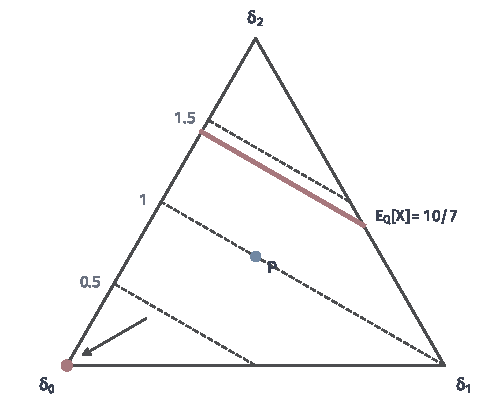
\includegraphics[width=84mm]{figures/07-probability/07-distribution-optimization/matplotlib/dsel-three-requirements/figure.pdf}
 \caption{$\{0,1,2\}$上的三种要求。三角形中每一点是一张概率表。深灰虚线是期望成本$\mathbb{E}_{Q}[V]=q(1)+2q(2)$的等值线，标注为取值，箭头指向成本最小的顶点$\delta_0$（红点）；红色线段是满足$\mathbb{E}_{Q}[X]=10/7$的全部分布；蓝点是参考分布$P$。}
 \label{fig:dsel-three-requirements}
\end{BookInlineFigure}

本章研究的三类问题正是这样的组合：
\begin{enumerate}
 \item 不加等式约束，最小化期望成本加上偏离参考分布的代价$\tau D_{\mathrm{KL}}(Q\Vert P)$，$\tau>0$调节两者的比重；
 \item 要求$\mathbb{E}_{Q}[\bm{T}]=\bm{m}$，在满足要求的分布中最小化$D_{\mathrm{KL}}(Q\Vert P)$；
 \item 要求$\mathbb{E}_{Q}[\bm{T}]=\bm{m}$，在满足要求的分布中最大化熵。
\end{enumerate}
其中$\bm{T}:\mathcal{X}\to\mathbb{R}^{k}$是若干个指定的统计量，$\bm{m}\in\mathbb{R}^{k}$是它们的指定平均值。

\paragraph{允许的分布}
一般情形下，$\mathcal{X}$是可测空间，记其上全体概率测度为$\mathcal{P}(\mathcal{X})$。待选对象是$\mathcal{P}(\mathcal{X})$中的元素，但并非每个元素都能参加比较。候选集合$\mathcal{Q}\subseteq\mathcal{P}(\mathcal{X})$是问题的一部分，要逐项写明。

非负性与归一化看起来理所当然，计算时却最容易丢掉。在上面的例子里，若只解那两个线性方程，以$q(1)=t$为参数，得到
\[
 q(2)=\frac57-\frac t2,\qquad q(0)=\frac27-\frac t2 .
\]
取$t=1$，得到$(-\tfrac{3}{14},1,\tfrac{3}{14})$。它和为$1$，平均值也是$10/7$，但$q(0)<0$，不是概率表。只有$0\leq t\leq4/7$才合法。凡是用方程、公式或数值迭代得出的“分布”，都要回头核对这两条。

其次是支持。若$Q$在$P$概率为零的地方放了质量，即$Q$不绝对连续于$P$，则$D_{\mathrm{KL}}(Q\Vert P)=+\infty$。所以只要目标里含有$D_{\mathrm{KL}}(Q\Vert P)$，有意义的候选都满足$Q\ll P$：选出的分布可以删去参考分布的状态，但不能添加新的状态。

最后是可积性。期望成本$\mathbb{E}_{Q}[V]$与约束中的$\mathbb{E}_{Q}[\bm{T}]$都要求相应函数在$Q$下可积，否则目标或约束不是一个确定的实数。有限状态上这一条自动成立，可数或连续状态上必须单独检查。

\begin{definition}[分布优化问题]
\label{def:dsel-problem}
设$\mathcal{Q}\subseteq\mathcal{P}(\mathcal{X})$是候选集合，$J:\mathcal{Q}\to(-\infty,+\infty]$。称
\begin{equation}
 J^{*}=\inf_{Q\in\mathcal{Q}}J(Q)
 \label{eq:dsel-problem}
\end{equation}
为\term{分布优化问题}（distribution optimization problem）的最优值。若$Q^{*}\in\mathcal{Q}$满足$J(Q^{*})=J^{*}$，称$Q^{*}$为\term{最优分布}（optimal distribution）。
\end{definition}

定义把三件事分开了。$\mathcal{Q}$非空且$J$在其上有定义，问题才成立；$J^{*}$可能是有限数，也可能是$-\infty$；即使$J^{*}$有限，也可能没有任何$Q$达到它。这三件事在第~\ref{sec:dsel-checks}节逐一检查，这里先看第一件事为什么不能省略。

\paragraph{无穷量不能相减}
目标$\mathbb{E}_{Q}[V]+\tau D_{\mathrm{KL}}(Q\Vert P)$由两项相加。第二项总在$[0,+\infty]$中；第一项若不加限制，可以是$-\infty$。下面的例子中两项分别是$-\infty$和$+\infty$。取$\mathcal{X}=\{1,2,\dots\}$，参考分布与成本为
\[
 P(k)=2^{-k},\qquad V(k)=-k ,
\]
候选分布取$Q(k)=\dfrac{6}{\pi^{2}k^{2}}$。

期望成本是调和级数乘以负数：
\[
 \mathbb{E}_{Q}[V]=-\frac{6}{\pi^{2}}\sum_{k\geq1}\frac1k=-\infty .
\]
再看对数比。对每个$k$，
\[
 \ln\frac{Q(k)}{P(k)}=\ln\frac{6}{\pi^{2}}-2\ln k+k\ln2 .
\]
按$Q$平均时，前两项给出收敛级数，因为$\sum_k(\ln k)/k^{2}<\infty$；第三项给出$\ln2\sum_kkQ(k)=+\infty$。所以$D_{\mathrm{KL}}(Q\Vert P)=+\infty$，目标成了“$-\infty+\infty$”。

把两个级数逐项配对，似乎能得到一个有限数。取$\tau=1/\ln2$，记前$N$项的部分和为
\[
 C_N=\sum_{k\leq N}Q(k)V(k),\qquad K_N=\tau\sum_{k\leq N}Q(k)\ln\frac{Q(k)}{P(k)} .
\]
这时$\tau k\ln2=k$，与$V(k)=-k$恰好抵消，$C_N+K_N$收敛到约$-2.363$。但若把$C_N$与$K_{2N}$配对，多出的部分是$\frac{6}{\pi^{2}}\sum_{N<k\leq2N}\frac1k$，它趋于$\frac{6}{\pi^{2}}\ln2\approx0.421$，极限变成约$-1.941$。图~\ref{fig:dsel-undefined-objective}画出了这几条部分和曲线。

\begin{BookInlineFigure}
 \centering
 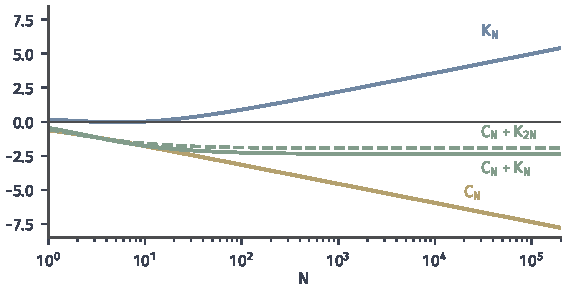
\includegraphics[width=96mm]{figures/07-probability/07-distribution-optimization/matplotlib/dsel-undefined-objective/figure.pdf}
 \caption{无定义的目标。$P(k)=2^{-k}$，$V(k)=-k$，$Q(k)=6/(\pi^{2}k^{2})$，$\tau=1/\ln2$，横轴为对数刻度。黄线是期望成本的部分和$C_N\to-\infty$，蓝线是KL项的部分和$K_N\to+\infty$；绿色实线$C_N+K_N$与绿色虚线$C_N+K_{2N}$各自收敛，极限相差$\frac{6}{\pi^{2}}\ln2\approx0.421$。}
 \label{fig:dsel-undefined-objective}
\end{BookInlineFigure}

一个数值若取决于怎样配对两条发散级数，它就不是目标函数的值。所以凡是目标含$\mathbb{E}_{Q}[V]+\tau D_{\mathrm{KL}}(Q\Vert P)$的问题，本章都把候选集合取为
\begin{equation}
 \mathcal{Q}_V=\Bigl\{Q\in\mathcal{P}(\mathcal{X}):\ D_{\mathrm{KL}}(Q\Vert P)<\infty,\ \mathbb{E}_{Q}\lvert V\rvert<\infty\Bigr\}.
 \label{eq:dsel-candidate-set}
\end{equation}
在$\mathcal{Q}_V$上两项都是有限实数，和有确定的值。有限状态且$P$处处为正时，$\mathcal{Q}_V$就是全部概率表。


\section{KL正则化的成本最小化}
\label{sec:dsel-kl-cost}

只降低期望成本，会把全部质量推到成本最低的状态上。若参考分布$P$代表原有的规律，我们愿意为降低成本而改动它，但改动本身也要付出代价。把这个代价记为$\tau D_{\mathrm{KL}}(Q\Vert P)$，$\tau>0$是一个换算系数：偏离参考分布一个nat，相当于多付$\tau$个单位的成本。

设$V:\mathcal{X}\to\mathbb{R}$可测，在每一点取有限值。在式~\eqref{eq:dsel-candidate-set}的候选集合上考虑
\begin{equation}
 \min_{Q\in\mathcal{Q}_V}\ J_\tau(Q),\qquad J_\tau(Q)=\mathbb{E}_{Q}[V]+\tau D_{\mathrm{KL}}(Q\Vert P).
 \label{eq:dsel-kl-cost-problem}
\end{equation}
在目标上加一个KL项以约束解不要离参考分布太远，这种做法称为\term{KL正则化}（KL regularization）。

\paragraph{有限状态上的权衡}
先在有限的$\mathcal{X}$上、$p(x)>0$处处成立时看目标的形状。这时
\[
 J_\tau(Q)=\sum_{x}q(x)V(x)+\tau\sum_{x}q(x)\ln\frac{q(x)}{p(x)} .
\]
第一项是线性的，它把质量拉向成本低的状态。第二项是凸的，而且函数$t\mapsto t\ln t$在$t\downarrow0$处的导数趋于$-\infty$：把某个状态的概率压到零，代价增长得极快。两者相抗，最优解应当留在三角形内部。

在内部，可以用归一化约束的Lagrange乘子$\nu$形式地求驻点。对$q(x)$求偏导并令其为零，得到
\[
 V(x)+\tau\Bigl(\ln\frac{q(x)}{p(x)}+1\Bigr)-\nu=0 .
\]
解出$q(x)$，
\[
 q(x)=p(x)\,\mathrm{e}^{-V(x)/\tau}\,\mathrm{e}^{\nu/\tau-1} .
\]
最后一个因子与$x$无关，由归一化确定。记$Z=\sum_xp(x)\mathrm{e}^{-V(x)/\tau}$，于是候选解是
\[
 q(x)=\frac{p(x)\,\mathrm{e}^{-V(x)/\tau}}{Z} .
\]
每个状态的参考概率乘上一个只由它自己的成本决定的权重$\mathrm{e}^{-V(x)/\tau}$，再整体归一。这一推导假设了解在内部且可微，只是猜测，下面将不借助导数直接验证它。

回到例子：$P$均匀，$V(x)=x$。取$\tau=1/\ln2$，权重就是$\mathrm{e}^{-V/\tau}=2^{-x}$，成本每多一个单位，权重减半。三个状态未归一的质量与归一化常数为
\[
 \frac13,\quad\frac16,\quad\frac1{12};\qquad Z=\frac13+\frac16+\frac1{12}=\frac7{12} .
\]
除以$Z$，得到
\[
 Q^{*}=\Bigl(\frac47,\ \frac27,\ \frac17\Bigr).
\]
图~\ref{fig:dsel-gibbs-bars}画出这一步：先乘权重，再归一化，质量从高成本状态挪向低成本状态，但没有任何状态被删去。

\begin{BookInlineFigure}
 \centering
 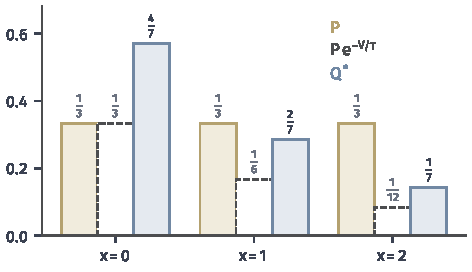
\includegraphics[width=80mm]{figures/07-probability/07-distribution-optimization/matplotlib/dsel-gibbs-bars/figure.pdf}
 \caption{按成本重新加权。$P$均匀（黄），$V(x)=x$，$\tau=1/\ln2$。白色虚线柱是未归一的$P\,\mathrm{e}^{-V/\tau}$，和为$Z=7/12$；蓝色柱是归一化后的$Q^{*}=(\frac47,\frac27,\frac17)$。}
 \label{fig:dsel-gibbs-bars}
\end{BookInlineFigure}

验证这个分布确实比别的好，先算它的目标值。期望成本是
\[
 \mathbb{E}_{Q^{*}}[V]=0\cdot\frac47+1\cdot\frac27+2\cdot\frac17=\frac47 .
\]
$P$的每个概率都是$1/3$，所以对数比是$\ln(3q^{*}(x))$，KL项为
\[
 D_{\mathrm{KL}}(Q^{*}\Vert P)=\frac47\ln\frac{12}7+\frac27\ln\frac67+\frac17\ln\frac37\approx0.3080-0.0440-0.1210=0.1429 .
\]
乘以$\tau=1/\ln2$后，KL项约为$0.2062$，相当于以比特计的偏离量。两项相加，
\[
 J_\tau(Q^{*})\approx0.5714+0.2062=0.7776 .
\]
对照两个极端：$\delta_0$的成本为零但偏离为$\ln3$，$P$的偏离为零但成本为$1$，
\[
 J_\tau(\delta_0)=\log_23\approx1.585,\qquad J_\tau(P)=1 .
\]
两者都比$Q^{*}$差。

\paragraph{参数$\tau$的作用}
$\tau$越小，偏离越便宜，解越接近只看成本的答案；$\tau$越大，偏离越贵，解越接近$P$。在例子中，$Q^{*}_\tau\propto\mathrm{e}^{-x/\tau}$。$\tau=0.5$时它约为$(0.867,0.117,0.016)$，$\tau=4$时约为$(0.419,0.326,0.254)$。$\tau\to0$时，权重$\mathrm{e}^{-x/\tau}$在$x=1,2$处趋于零，在$x=0$处恒为$1$，所以$Q^{*}_\tau\to\delta_0$；$\tau\to\infty$时三个权重都趋于$1$，$Q^{*}_\tau\to P$。图~\ref{fig:dsel-gibbs-path}画出这条从$\delta_0$到$P$的路径。

\begin{BookInlineFigure}
 \centering
 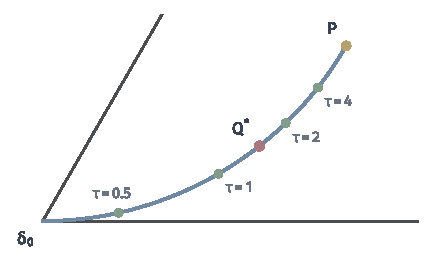
\includegraphics[width=72mm]{figures/07-probability/07-distribution-optimization/matplotlib/dsel-gibbs-path/figure.pdf}
 \caption{$\tau$从$0$增大到$\infty$时，$Q^{*}_\tau\propto P\,\mathrm{e}^{-V/\tau}$在概率三角形左下部分走过的路径（蓝），$P$均匀，$V(x)=x$。绿点依次是$\tau=0.5,1,2,4$，红点是$\tau=1/\ln2$时的$(\frac47,\frac27,\frac17)$，黄点是$P$。}
 \label{fig:dsel-gibbs-path}
\end{BookInlineFigure}

换一个角度看这个权衡。每个候选$Q$对应平面上的一点，横坐标是偏离$D_{\mathrm{KL}}(Q\Vert P)$，纵坐标是期望成本$\mathbb{E}_{Q}[V]$。目标$J_\tau$的等值线是斜率为$-\tau$的直线
\[
 \mathbb{E}_{Q}[V]=c-\tau D_{\mathrm{KL}}(Q\Vert P) .
\]
最小化$J_\tau$，就是把这条直线向下平移，直到它刚好碰到所有候选点组成的区域。图~\ref{fig:dsel-tradeoff}中，碰到的点正是$Q^{*}$；不同的$\tau$给出不同的斜率，碰到区域下边界上不同的点，而整条下边界就是上面那条Gibbs路径。下面的定理会证明这一点。

\begin{BookInlineFigure}
 \centering
 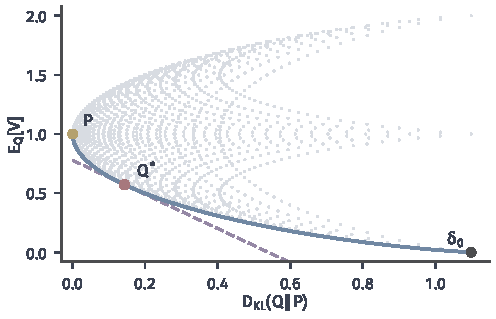
\includegraphics[width=84mm]{figures/07-probability/07-distribution-optimization/matplotlib/dsel-tradeoff/figure.pdf}
 \caption{成本与偏离的权衡，$P$均匀，$V(x)=x$。浅灰点是概率三角形中步长$1/60$的格点分布对应的$\bigl(D_{\mathrm{KL}}(Q\Vert P),\mathbb{E}_{Q}[V]\bigr)$；蓝线是Gibbs路径，它是可达区域的下边界。紫色虚线是$\tau=1/\ln2$时目标的等值线$\mathbb{E}_{Q}[V]=J^{*}-\tau D_{\mathrm{KL}}(Q\Vert P)$，在红点$Q^{*}$处与边界相切。}
 \label{fig:dsel-tradeoff}
\end{BookInlineFigure}

\paragraph{Gibbs分布的最优性}
有限状态上的形式推导提示了一般的答案：把$P$按$\mathrm{e}^{-V/\tau}$重新加权。下面在一般可测空间上定义它，并直接证明它的最优性。

\begin{definition}[Gibbs分布]
\label{def:dsel-gibbs}
设$P\in\mathcal{P}(\mathcal{X})$，$V:\mathcal{X}\to\mathbb{R}$可测，$\tau>0$，且
\begin{equation}
 Z=\mathbb{E}_{P}\bigl[\mathrm{e}^{-V/\tau}\bigr]<\infty .
 \label{eq:dsel-gibbs-partition}
\end{equation}
以
\begin{equation}
 \frac{\mathrm{d}Q^{*}_\tau}{\mathrm{d}P}=\frac{\mathrm{e}^{-V/\tau}}{Z}
 \label{eq:dsel-gibbs}
\end{equation}
定义的概率测度$Q^{*}_\tau$称为成本$V$、参数$\tau$相对于$P$的\term{Gibbs分布}（Gibbs distribution）。
\end{definition}

被积函数$\mathrm{e}^{-V/\tau}$处处为正，所以$Z>0$总成立，式~\eqref{eq:dsel-gibbs-partition}中真正的条件是$Z$有限。密度$\mathrm{e}^{-V/\tau}/Z$处处为正且有限，因此$Q^{*}_\tau$与$P$互相绝对连续：二者的零概率事件完全相同。

\begin{theorem}[Gibbs变分原理]
\label{thm:dsel-gibbs-variational}
设$V:\mathcal{X}\to\mathbb{R}$可测，$\tau>0$，$Z=\mathbb{E}_{P}[\mathrm{e}^{-V/\tau}]<\infty$，$Q^{*}=Q^{*}_\tau$为式~\eqref{eq:dsel-gibbs}的Gibbs分布。
\begin{enumerate}
 \item 对每个$Q\in\mathcal{Q}_V$，
 \begin{equation}
 J_\tau(Q)=-\tau\ln Z+\tau D_{\mathrm{KL}}(Q\Vert Q^{*}) .
 \label{eq:dsel-gibbs-identity}
 \end{equation}
 特别地，$J_\tau(Q)\geq-\tau\ln Z$。
 \item 若还有$\mathbb{E}_{Q^{*}}\lvert V\rvert<\infty$，则$Q^{*}\in\mathcal{Q}_V$，$J_\tau(Q^{*})=-\tau\ln Z$，并且$Q^{*}$是问题~\eqref{eq:dsel-kl-cost-problem}的唯一最优分布。
\end{enumerate}
\end{theorem}

\begin{proof}
第一部分。设$Q\in\mathcal{Q}_V$。由$D_{\mathrm{KL}}(Q\Vert P)<\infty$知$Q\ll P$；$P$与$Q^{*}$互相绝对连续，所以$Q\ll Q^{*}$。由密度的链式法则与式~\eqref{eq:dsel-gibbs}，$Q$几乎处处有
\[
 \frac{\mathrm{d}Q}{\mathrm{d}Q^{*}}=\frac{\mathrm{d}Q}{\mathrm{d}P}\cdot\frac{\mathrm{d}P}{\mathrm{d}Q^{*}}=\frac{\mathrm{d}Q}{\mathrm{d}P}\cdot Z\,\mathrm{e}^{V/\tau} .
\]
取对数，
\[
 \ln\frac{\mathrm{d}Q}{\mathrm{d}Q^{*}}=\ln\frac{\mathrm{d}Q}{\mathrm{d}P}+\frac{V}{\tau}+\ln Z .
\]

右边每一项都在$Q$下可积：$D_{\mathrm{KL}}(Q\Vert P)$有限，而对数比的负部总是可积的，所以$\ln(\mathrm{d}Q/\mathrm{d}P)$在$Q$下可积；$V$在$Q$下可积是$\mathcal{Q}_V$的定义；$\ln Z$是常数。于是可以对右边逐项取$Q$下的期望，左边的期望就是$D_{\mathrm{KL}}(Q\Vert Q^{*})$：
\[
 D_{\mathrm{KL}}(Q\Vert Q^{*})=D_{\mathrm{KL}}(Q\Vert P)+\frac{1}{\tau}\mathbb{E}_{Q}[V]+\ln Z .
\]
两边乘以$\tau$并移项，即得式~\eqref{eq:dsel-gibbs-identity}。由Gibbs不等式$D_{\mathrm{KL}}(Q\Vert Q^{*})\geq0$，得到$J_\tau(Q)\geq-\tau\ln Z$。

第二部分。由式~\eqref{eq:dsel-gibbs}，$\ln(\mathrm{d}Q^{*}/\mathrm{d}P)=-V/\tau-\ln Z$。当$V$在$Q^{*}$下可积时，它在$Q^{*}$下可积，
\[
 D_{\mathrm{KL}}(Q^{*}\Vert P)=-\frac1\tau\mathbb{E}_{Q^{*}}[V]-\ln Z<\infty ,
\]
所以$Q^{*}\in\mathcal{Q}_V$。在式~\eqref{eq:dsel-gibbs-identity}中取$Q=Q^{*}$，得到$J_\tau(Q^{*})=-\tau\ln Z$，它等于第一部分给出的下界，所以$Q^{*}$最优。若另一个$Q\in\mathcal{Q}_V$也达到这个值，则$D_{\mathrm{KL}}(Q\Vert Q^{*})=0$，由Gibbs不等式的等号条件$Q=Q^{*}$。
\end{proof}

定理~\ref{thm:dsel-gibbs-variational}称为\term{Gibbs变分原理}（Gibbs variational principle）。式~\eqref{eq:dsel-gibbs-identity}比“$Q^{*}$最优”说得更多：任何候选的目标值比最优值多出的部分，恰好是$\tau D_{\mathrm{KL}}(Q\Vert Q^{*})$。在例子中，$J_\tau(P)-J_\tau(Q^{*})\approx1-0.7776=0.2224$，而直接计算
\[
 \tau D_{\mathrm{KL}}(P\Vert Q^{*})=\frac{1}{3\ln2}\ln\Bigl(\frac{7}{12}\cdot\frac76\cdot\frac73\Bigr)=\frac13\log_2\frac{343}{216}\approx0.2224 ,
\]
两者一致。这个恒等式把“离最优还差多少”变成一个可以计算的散度，第~\ref{sec:dsel-checks}节将用它检验数值解。

最优值$-\tau\ln\mathbb{E}_{P}[\mathrm{e}^{-V/\tau}]$也有清楚的含义。令$g=-V/\tau$，第一部分可以改写为：对每个$Q\in\mathcal{Q}_V$，
\begin{equation}
 \mathbb{E}_{Q}[g]\leq D_{\mathrm{KL}}(Q\Vert P)+\ln\mathbb{E}_{P}\bigl[\mathrm{e}^{g}\bigr] ,
 \label{eq:dsel-dv}
\end{equation}
第~\ref{chap:distribution-comparison}章用这个不等式由KL散度控制期望差。定理的第二部分说明它不能再改进：当$\mathbb{E}_{Q^{*}}\lvert g\rvert<\infty$时，等号在指数倾斜$Q^{*}$处取到，于是
\[
 \ln\mathbb{E}_{P}\bigl[\mathrm{e}^{g}\bigr]=\max_{Q\in\mathcal{Q}_V}\Bigl\{\mathbb{E}_{Q}[g]-D_{\mathrm{KL}}(Q\Vert P)\Bigr\} .
\]
对数矩母函数是“期望减去偏离代价”在全体候选上的最大值。

Gibbs分布的形式不是事先选定的分布族，而是由目标推出来的。它是$P$沿统计量$V$、以参数$-1/\tau$作的指数倾斜，属于第~\ref{chap:distribution-families}章以$P$为基准测度、以$V$为自然统计量的指数族。

由定理还可以读出图~\ref{fig:dsel-tradeoff}中的下边界。设$Q\in\mathcal{Q}_V$的偏离不超过$Q^{*}$的偏离，即
\[
 D_{\mathrm{KL}}(Q\Vert P)\leq D_{\mathrm{KL}}(Q^{*}\Vert P) .
\]
由$J_\tau(Q)\geq J_\tau(Q^{*})$，
\[
 \begin{aligned}
 \mathbb{E}_{Q}[V]&\geq\mathbb{E}_{Q^{*}}[V]+\tau\bigl(D_{\mathrm{KL}}(Q^{*}\Vert P)-D_{\mathrm{KL}}(Q\Vert P)\bigr)\\
 &\geq\mathbb{E}_{Q^{*}}[V] .
 \end{aligned}
\]
也就是说，在不超过$Q^{*}$的偏离预算下，没有哪个分布的期望成本更低。

\paragraph{配分函数无穷时}
条件$Z<\infty$不是技术细节。回到第~\ref{sec:dsel-problems}节的可数例子：$P(k)=2^{-k}$，$V(k)=-k$，$k\geq1$。记$r=\mathrm{e}^{1/\tau}/2$，则
\[
 Z(\tau)=\sum_{k\geq1}2^{-k}\mathrm{e}^{k/\tau}=\sum_{k\geq1}r^{k} .
\]
它有限当且仅当$r<1$，即$\tau>1/\ln2$；这时$Z=r/(1-r)$，Gibbs分布$Q^{*}(k)=(1-r)r^{k-1}$是几何分布，$\mathbb{E}_{Q^{*}}\lvert V\rvert=1/(1-r)$有限，定理~\ref{thm:dsel-gibbs-variational}的两部分都适用。例如$\tau=2$时，$r\approx0.8244$，$Z\approx4.693$，最优值$-2\ln Z\approx-3.092$。

$\tau\leq1/\ln2$时没有Gibbs分布，最优值是$-\infty$。取$Q_N$为$\{1,\dots,N\}$上的均匀分布，它的期望成本与KL散度分别是
\[
 \begin{gathered}
 \mathbb{E}_{Q_N}[V]=-\frac{N+1}{2},\\
 D_{\mathrm{KL}}(Q_N\Vert P)=\frac1N\sum_{k=1}^{N}\bigl(k\ln2-\ln N\bigr)=\frac{(N+1)\ln2}{2}-\ln N .
 \end{gathered}
\]
代入目标，
\[
 J_\tau(Q_N)=\frac{N+1}{2}\bigl(\tau\ln2-1\bigr)-\tau\ln N .
\]
$\tau\ln2\leq1$时第一项不为正，第二项趋于$-\infty$，所以$J_\tau(Q_N)\to-\infty$。远处状态带来的收益$k$增长得不比偏离的代价$\tau k\ln2$慢，把质量往远处推永远划算。图~\ref{fig:dsel-partition-threshold}画出这一转变。

\begin{BookInlineFigure}
 \centering
 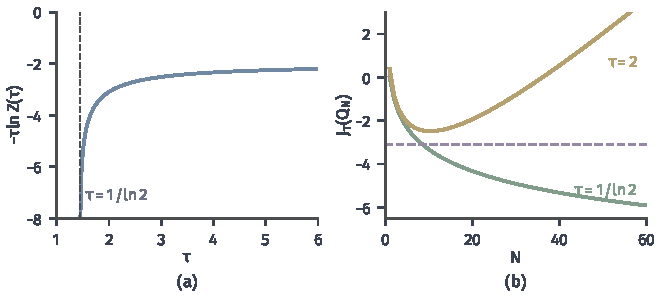
\includegraphics[width=112mm]{figures/07-probability/07-distribution-optimization/matplotlib/dsel-partition-threshold/figure.pdf}
 \caption{配分函数的有限性。$P(k)=2^{-k}$，$V(k)=-k$。(a)最优值$-\tau\ln Z(\tau)$（蓝），$\tau\downarrow1/\ln2$（深灰虚线）时趋于$-\infty$。(b)$\{1,\dots,N\}$上均匀分布$Q_N$的目标值：$\tau=1/\ln2$时（绿）等于$-\log_2N$，无下界；$\tau=2$时（黄）始终高于最优值$-2\ln Z(2)\approx-3.092$（紫色虚线）。}
 \label{fig:dsel-partition-threshold}
\end{BookInlineFigure}

定理第二部分的条件$\mathbb{E}_{Q^{*}}\lvert V\rvert<\infty$也可能不成立。那时$Z$有限，第一部分的恒等式仍然给出下界$-\tau\ln Z$，可是写出来的$Q^{*}$不在候选集合中。这种情形放到第~\ref{sec:dsel-checks}节，与“最小值是否被达到”一起讨论。


\section{矩约束下的最小KL}
\label{sec:dsel-min-kl}

上一节的成本是“软”的：成本可以高一点，只要偏离小一点。另一类要求是“硬”的：选出的分布必须满足某些平均量，例如平均点数必须是$10/7$。满足要求的分布在图~\ref{fig:dsel-three-requirements}中排成一条线段，我们要在这条线段上挑出离参考分布最近的一个。

设$\bm{T}:\mathcal{X}\to\mathbb{R}^{k}$可测，$\bm{m}\in\mathbb{R}^{k}$。满足矩要求的分布组成集合
\[
 \mathcal{C}_{\bm{m}}=\Bigl\{Q\in\mathcal{P}(\mathcal{X}):\ \mathbb{E}_{Q}\lVert\bm{T}\rVert_2<\infty,\ \mathbb{E}_{Q}[\bm{T}]=\bm{m}\Bigr\}.
\]
本节研究
\begin{equation}
 \min_{Q\in\mathcal{C}_{\bm{m}}}\ D_{\mathrm{KL}}(Q\Vert P) .
 \label{eq:dsel-min-kl-problem}
\end{equation}
所有能由$P$的绝对连续分布实现的矩组成\term{可行矩集合}（set of feasible moments）
\[
 \mathcal{M}=\Bigl\{\mathbb{E}_{Q}[\bm{T}]:\ Q\ll P,\ \mathbb{E}_{Q}\lVert\bm{T}\rVert_2<\infty\Bigr\}.
\]
只有$\bm{m}\in\mathcal{M}$时问题~\eqref{eq:dsel-min-kl-problem}才有KL有限的候选。

KL的方向在这里是$D_{\mathrm{KL}}(Q\Vert P)$：期望按待选的$Q$计算，有限的前提是$Q\ll P$。所以选出的分布可以删去$P$的某些状态，却不会在$P$认为不可能的地方放质量。参考分布代表原有的认识，矩要求是新加的条件，问题问的是：为了满足新条件，最少要把原有认识改动多少。若反过来最小化$D_{\mathrm{KL}}(P\Vert Q)$，期望按$P$计算，要求$Q$覆盖$P$的全部状态，这对应另一类问题，在第~\ref{chap:distribution-approximation}章讨论。

\subsection{指数倾斜}
\label{sec:dsel-tilt}

先在有限状态上求解。设$\mathcal{X}$有限，$p(x)>0$对每个$x$成立。这时每个$Q$都绝对连续于$P$，$Q$的矩是$\bm{T}(x)$的凸组合，而任何凸组合也都能由某个$Q$实现，所以
\[
 \mathcal{M}=\operatorname{conv}\{\bm{T}(x):x\in\mathcal{X}\}
\]
是有限个点的凸包。在例子中$T(x)=x$，$\mathcal{M}=[0,2]$。

\paragraph{乘子方程}
在概率三角形内部形式地求驻点。对归一化引入乘子$\nu$，对矩约束引入乘子向量$\bm{\theta}\in\mathbb{R}^{k}$，Lagrange函数为
\[
 \sum_xq(x)\ln\frac{q(x)}{p(x)}-\Bigl\langle\bm{\theta},\sum_xq(x)\bm{T}(x)-\bm{m}\Bigr\rangle-\nu\Bigl(\sum_xq(x)-1\Bigr).
\]
对$q(x)$求偏导并令其为零，得到
\[
 \ln\frac{q(x)}{p(x)}+1-\langle\bm{\theta},\bm{T}(x)\rangle-\nu=0 .
\]

解出
\[
 q(x)=p(x)\exp\bigl(\langle\bm{\theta},\bm{T}(x)\rangle\bigr)\,\mathrm{e}^{\nu-1} ,
\]
再由归一化定出常数因子：
\begin{equation}
 q_{\bm{\theta}}(x)=p(x)\exp\bigl(\langle\bm{\theta},\bm{T}(x)\rangle-A(\bm{\theta})\bigr),\qquad A(\bm{\theta})=\ln\sum_xp(x)\,\mathrm{e}^{\langle\bm{\theta},\bm{T}(x)\rangle} .
 \label{eq:dsel-tilt-finite}
\end{equation}
乘子$\bm{\theta}$还没有确定，它要使$q_{\bm{\theta}}$满足矩约束。Lagrange乘子法给出的是必要条件的形式（见\BookChapterRef{chap:constrained-optimality}{卷五第17章“约束问题的最优性”}），这里又假设了解在内部，所以式~\eqref{eq:dsel-tilt-finite}仍只是候选。

这个形式在一般空间上同样有意义。

\begin{definition}[指数倾斜]
\label{def:dsel-tilt}
设$P\in\mathcal{P}(\mathcal{X})$，$\bm{\theta}\in\mathbb{R}^{k}$，并且
\begin{equation}
 A(\bm{\theta})=\ln\mathbb{E}_{P}\bigl[\mathrm{e}^{\langle\bm{\theta},\bm{T}\rangle}\bigr]<\infty .
 \label{eq:dsel-tilt-partition}
\end{equation}
以
\begin{equation}
 \frac{\mathrm{d}Q_{\bm{\theta}}}{\mathrm{d}P}=\exp\bigl(\langle\bm{\theta},\bm{T}\rangle-A(\bm{\theta})\bigr)
 \label{eq:dsel-tilt}
\end{equation}
定义的$Q_{\bm{\theta}}$称为$P$沿$\bm{T}$的\term{指数倾斜}（exponential tilting）。
\end{definition}

全体$Q_{\bm{\theta}}$就是第~\ref{chap:distribution-families}章以$P$为基准测度、以$\bm{T}$为自然统计量的指数族，$A$是它的对数配分函数。密度处处为正，所以每个$Q_{\bm{\theta}}$与$P$互相绝对连续。在例子中，$P$均匀，$T(x)=x$，$q_\theta(x)\propto\mathrm{e}^{\theta x}$。取$\theta=\ln2$，三个权重是$1,2,4$，
\[
 Q_{\ln2}=\Bigl(\frac17,\ \frac27,\ \frac47\Bigr),\qquad\mathbb{E}_{Q_{\ln2}}[X]=\frac{2+8}{7}=\frac{10}{7},
\]
它恰好落在约束线段上。

\paragraph{勾股恒等式}
要说明$Q_{\ln2}$比线段上其他分布更接近$P$，不必求导，只需把$D_{\mathrm{KL}}(Q\Vert P)$拆开，得到下面的\term{勾股恒等式}。

\begin{lemma}[勾股恒等式]
\label{lem:dsel-pythagoras}
设$A(\bm{\theta})<\infty$，$Q\in\mathcal{C}_{\bm{m}}$且$D_{\mathrm{KL}}(Q\Vert P)<\infty$。则
\begin{equation}
 D_{\mathrm{KL}}(Q\Vert P)=D_{\mathrm{KL}}(Q\Vert Q_{\bm{\theta}})+\langle\bm{\theta},\bm{m}\rangle-A(\bm{\theta}) .
 \label{eq:dsel-pythagoras-general}
\end{equation}
若$Q_{\bm{\theta}}$本身也属于$\mathcal{C}_{\bm{m}}$，则
\begin{equation}
 D_{\mathrm{KL}}(Q\Vert P)=D_{\mathrm{KL}}(Q\Vert Q_{\bm{\theta}})+D_{\mathrm{KL}}(Q_{\bm{\theta}}\Vert P) .
 \label{eq:dsel-pythagoras}
\end{equation}
\end{lemma}

\begin{proof}
$Q\ll P$，而$P$与$Q_{\bm{\theta}}$互相绝对连续，所以$Q\ll Q_{\bm{\theta}}$。由链式法则与式~\eqref{eq:dsel-tilt}，
\[
 \ln\frac{\mathrm{d}Q}{\mathrm{d}Q_{\bm{\theta}}}=\ln\frac{\mathrm{d}Q}{\mathrm{d}P}-\langle\bm{\theta},\bm{T}\rangle+A(\bm{\theta}) .
\]
右边第一项在$Q$下可积（KL有限，负部总可积），第二项因$\mathbb{E}_{Q}\lVert\bm{T}\rVert_2<\infty$可积。逐项取$Q$下的期望，并用$\mathbb{E}_{Q}[\bm{T}]=\bm{m}$，
\[
 D_{\mathrm{KL}}(Q\Vert Q_{\bm{\theta}})=D_{\mathrm{KL}}(Q\Vert P)-\langle\bm{\theta},\bm{m}\rangle+A(\bm{\theta}) ,
\]
移项即得式~\eqref{eq:dsel-pythagoras-general}。若$Q_{\bm{\theta}}\in\mathcal{C}_{\bm{m}}$，则式~\eqref{eq:dsel-tilt}给出的对数密度在$Q_{\bm{\theta}}$下可积，其期望是
\[
 D_{\mathrm{KL}}(Q_{\bm{\theta}}\Vert P)=\langle\bm{\theta},\bm{m}\rangle-A(\bm{\theta}) .
\]
代回式~\eqref{eq:dsel-pythagoras-general}即得式~\eqref{eq:dsel-pythagoras}。
\end{proof}

证明的关键一步是：$\ln(\mathrm{d}Q_{\bm{\theta}}/\mathrm{d}P)$只通过$\bm{T}$依赖于$x$，而约束集合中所有分布的$\bm{T}$平均值都相同，所以这个对数比在约束集合上的平均是常数。

在例子中验证。取线段的一个端点$Q=(\tfrac27,0,\tfrac57)$，三个散度分别是
\[
 \begin{gathered}
 D_{\mathrm{KL}}(Q\Vert P)=\tfrac27\ln\tfrac67+\tfrac57\ln\tfrac{15}7\approx0.5003,\\
 D_{\mathrm{KL}}(Q\Vert Q_{\ln2})=\tfrac27\ln2+\tfrac57\ln\tfrac54\approx0.3574,\qquad D_{\mathrm{KL}}(Q_{\ln2}\Vert P)\approx0.1429 .
 \end{gathered}
\]
后两项之和正是第一项。图~\ref{fig:dsel-pythagoras}把这三个量画成一个“直角三角形”：约束集合是一条直线，倾斜族是与它相交的曲线，交点$Q_{\ln2}$像是垂足。

\begin{BookInlineFigure}
 \centering
 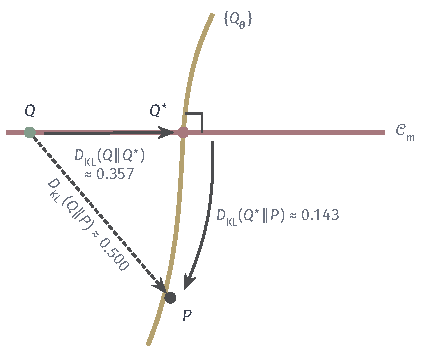
\includegraphics[width=72mm]{figures/07-probability/07-distribution-optimization/tikz/dsel-pythagoras/figure.pdf}
 \caption{勾股恒等式的示意。红线是约束集合$\mathcal{C}_{\bm{m}}$，黄线是倾斜族$\{Q_{\bm{\theta}}\}$，两者交于$Q^{*}=Q_{\ln2}$。箭头从KL的第一个分布指向第二个分布，数值取自$P$均匀、$T(x)=x$、$m=10/7$、$Q=(\frac27,0,\frac57)$的例子，单位为nat。}
 \label{fig:dsel-pythagoras}
\end{BookInlineFigure}

这个“勾股”只是类比。KL散度不对称，也不满足三角不等式，恒等式~\eqref{eq:dsel-pythagoras}只在一个点位于约束集合、另一个点是满足同一约束的倾斜分布时成立。三角形中实际的几何如图~\ref{fig:dsel-kl-projection}：以$P$为中心的KL等值线一圈圈向外扩张，第一次碰到约束线段的地方就是$Q_{\ln2}$，倾斜族的曲线恰好从这一点穿过。

\begin{BookInlineFigure}
 \centering
 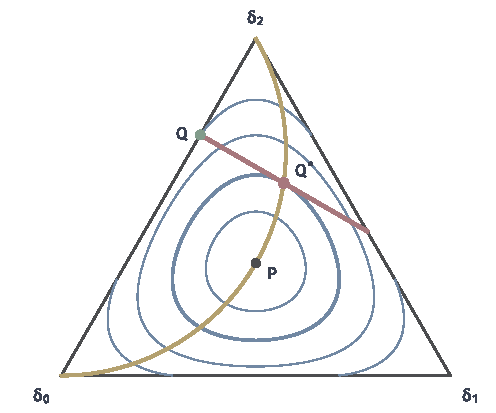
\includegraphics[width=84mm]{figures/07-probability/07-distribution-optimization/matplotlib/dsel-kl-projection/figure.pdf}
 \caption{约束线段上离$P$最近的分布。蓝线是$D_{\mathrm{KL}}(Q\Vert P)$的等值线，取值$0.05,0.3,0.5$（细）与最小值$D^{*}\approx0.1429$（粗）；红色线段是$\mathbb{E}_{Q}[X]=10/7$；黄线是倾斜族$q_\theta\propto\mathrm{e}^{\theta x}$。粗等值线在红点$Q^{*}=(\frac17,\frac27,\frac47)$处与线段相切；绿点$Q=(\frac27,0,\frac57)$满足约束，但落在更外圈。}
 \label{fig:dsel-kl-projection}
\end{BookInlineFigure}

\paragraph{最优性与存在性}
引理把最优性归结为一件事：能否找到$\bm{\theta}$，使$Q_{\bm{\theta}}$满足约束。这需要$\bm{m}$离可行矩集合的边界有一段距离。可行矩集合可能是低维的，例如当所有$\bm{T}(x)$都落在$\mathbb{R}^{2}$的一条直线上时，$\mathcal{M}$是一条线段，它在平面中没有内点。所以“远离边界”要在$\mathcal{M}$所在的仿射包$\operatorname{aff}\mathcal{M}$内衡量：$\bm{m}$属于$\mathcal{M}$的相对内部$\operatorname{ri}\mathcal{M}$，是指存在$\varepsilon>0$，使$\operatorname{aff}\mathcal{M}$中与$\bm{m}$距离小于$\varepsilon$的点都在$\mathcal{M}$中。上面的线段，相对内部就是去掉两个端点。

\begin{theorem}[指数倾斜给出最小KL]
\label{thm:dsel-min-kl}
设$\mathcal{X}$有限，$p(x)>0$对每个$x$成立，$\bm{m}\in\operatorname{ri}\mathcal{M}$。则
\begin{enumerate}
 \item 存在$\bm{\theta}^{*}\in\mathbb{R}^{k}$，使$\mathbb{E}_{Q_{\bm{\theta}^{*}}}[\bm{T}]=\bm{m}$；
 \item $Q^{*}=Q_{\bm{\theta}^{*}}$是问题~\eqref{eq:dsel-min-kl-problem}的唯一最优分布，最优值为
 \begin{equation}
 D^{*}=\langle\bm{\theta}^{*},\bm{m}\rangle-A(\bm{\theta}^{*}) ;
 \label{eq:dsel-min-kl-value}
 \end{equation}
 \item 满足第一条的$\bm{\theta}^{*}$可能不唯一，但它们给出同一个$Q^{*}$。
\end{enumerate}
\end{theorem}

\begin{proof}
第一部分。令
\[
 \ell(\bm{\theta})=\langle\bm{\theta},\bm{m}\rangle-A(\bm{\theta}) ,
\]
我们证明它有最大值点，并且最大值点满足矩约束。把$\ell$写成
\[
 -\ell(\bm{\theta})=\ln\sum_xp(x)\,\mathrm{e}^{\langle\bm{\theta},\bm{T}(x)-\bm{m}\rangle} .
\]
记
\[
 L=\operatorname{span}\{\bm{T}(x)-\bm{m}:x\in\mathcal{X}\} .
\]
因为$\bm{m}\in\mathcal{M}$，有$\operatorname{aff}\mathcal{M}=\bm{m}+L$。若$\bm{a}\perp L$，则每个指数中$\langle\bm{a},\bm{T}(x)-\bm{m}\rangle=0$，所以$\ell(\bm{\theta}+\bm{a})=\ell(\bm{\theta})$。只需在子空间$L$上找最大值点。

对$L$中的单位向量$\bm{u}$，令
\[
 \delta(\bm{u})=\max_{x\in\mathcal{X}}\langle\bm{u},\bm{T}(x)-\bm{m}\rangle .
\]
由于$\bm{m}\in\operatorname{ri}\mathcal{M}$，存在$\varepsilon>0$使$\bm{m}+\varepsilon\bm{u}\in\mathcal{M}$，即它是某个凸组合$\sum_xq(x)\bm{T}(x)$。与$\bm{u}$作内积，
\[
 \varepsilon=\sum_xq(x)\langle\bm{u},\bm{T}(x)-\bm{m}\rangle\leq\delta(\bm{u}) .
\]
所以$\delta(\bm{u})>0$。$\delta$在$L$的单位球面上连续，球面紧，于是$\delta_0=\min\delta(\bm{u})>0$。

对$\bm{\theta}\in L$，$\bm{\theta}\neq\bm{0}$，取$\bm{u}=\bm{\theta}/\lVert\bm{\theta}\rVert_2$。和式中至少有一项的指数是$\lVert\bm{\theta}\rVert_2\,\delta(\bm{u})$，其余各项为正，记$p_{\min}=\min_xp(x)>0$，得到
\[
 -\ell(\bm{\theta})\geq\ln p_{\min}+\delta_0\lVert\bm{\theta}\rVert_2 .
\]
所以$-\ell$在$L$上连续且当$\lVert\bm{\theta}\rVert_2\to\infty$时趋于$+\infty$，它在$L$的某个闭球上取到在$L$上的最小值，设最小值点为$\bm{\theta}^{*}$。由$\ell$沿$L^{\perp}$不变，$\bm{\theta}^{*}$也是$\ell$在整个$\mathbb{R}^{k}$上的最大值点。

$\ell$可微，最大值点处梯度为零。对式~\eqref{eq:dsel-tilt-finite}中的$A$求梯度，
\[
 \nabla A(\bm{\theta})=\frac{\sum_xp(x)\bm{T}(x)\mathrm{e}^{\langle\bm{\theta},\bm{T}(x)\rangle}}{\sum_xp(x)\mathrm{e}^{\langle\bm{\theta},\bm{T}(x)\rangle}}=\mathbb{E}_{Q_{\bm{\theta}}}[\bm{T}] .
\]
于是
\[
 \nabla\ell(\bm{\theta}^{*})=\bm{m}-\mathbb{E}_{Q_{\bm{\theta}^{*}}}[\bm{T}]=\bm{0} .
\]


第二部分。有限状态上每个$Q\in\mathcal{C}_{\bm{m}}$都满足$D_{\mathrm{KL}}(Q\Vert P)<\infty$。由引理~\ref{lem:dsel-pythagoras}，
\[
 D_{\mathrm{KL}}(Q\Vert P)=D_{\mathrm{KL}}(Q\Vert Q^{*})+D_{\mathrm{KL}}(Q^{*}\Vert P)\geq D_{\mathrm{KL}}(Q^{*}\Vert P),
\]
等号当且仅当$D_{\mathrm{KL}}(Q\Vert Q^{*})=0$，即$Q=Q^{*}$。最优值由引理中的表达式给出。

第三部分。若$\bm{\theta}^{*}$与$\bm{\theta}'$都满足矩约束，则$Q_{\bm{\theta}^{*}}$与$Q_{\bm{\theta}'}$都是最优分布，由唯一性二者相同。
\end{proof}

三个条件各有作用。$p(x)>0$保证每个候选都绝对连续于$P$；若$P$有零概率的状态，先把它们从$\mathcal{X}$中删去即可。有限性保证$A(\bm{\theta})$对一切$\bm{\theta}$有限，也提供了证明中的紧性。$\bm{m}\in\operatorname{ri}\mathcal{M}$保证存在有限的$\bm{\theta}^{*}$；第~\ref{sec:dsel-moment-matching}节会看到，$\bm{m}$在边界上时最优分布仍然存在，但不再是任何$Q_{\bm{\theta}}$。

在例子中，$\theta^{*}=\ln2$，$A(\ln2)=\ln\frac{1+2+4}{3}=\ln\frac73$，由式~\eqref{eq:dsel-min-kl-value}，
\[
 D^{*}=\frac{10}{7}\ln2-\ln\frac73\approx0.9902-0.8473=0.1429 ,
\]
与直接计算一致。

\paragraph{指数族从哪里来}
问题~\eqref{eq:dsel-min-kl-problem}的候选是$\mathcal{X}$上的全部分布，并没有限定在某个参数族中，最优解却落在以$P$为基准、以约束统计量$\bm{T}$为自然统计量的指数族里。Lagrange乘子变成了自然参数，要约束哪些平均量，就决定了用哪些统计量作指数权重。所以这一步不能理解为“先选一个指数族，再在族内近似”：族是最优性条件的产物。第~\ref{chap:distribution-approximation}章研究的是另一类问题，那里先限定候选族，再在族内逼近一个给定的目标分布。

上一节的Gibbs分布也是这样的解。取$\bm{T}=V$，$\bm{\theta}=-1/\tau$，Gibbs分布$Q^{*}_\tau$就是$P$沿$V$的倾斜；由定理~\ref{thm:dsel-min-kl}，它是所有满足$\mathbb{E}_{Q}[V]=\mathbb{E}_{Q^{*}_\tau}[V]$的分布中离$P$最近的一个。例如$(\tfrac47,\tfrac27,\tfrac17)$是平均成本为$4/7$的分布中KL最小者。成本加罚的软约束与矩的硬约束，在指数倾斜这里汇合。

\subsection{矩匹配}
\label{sec:dsel-moment-matching}

定理~\ref{thm:dsel-min-kl}把“选一个分布”变成了“解一个方程”：找$\bm{\theta}$使
\begin{equation}
 \nabla A(\bm{\theta})=\mathbb{E}_{Q_{\bm{\theta}}}[\bm{T}]=\bm{m} .
 \label{eq:dsel-moment-matching}
\end{equation}
这称为\term{矩匹配方程}（moment-matching equation）。未知数只有$k$个，与$\mathcal{X}$的大小无关。第~\ref{chap:distribution-families}章已经知道，在自然参数域内部$\nabla A$是均值映射，$A$的Hessian是统计量的协方差矩阵：
\[
 \nabla^{2}A(\bm{\theta})=\operatorname{Cov}_{Q_{\bm{\theta}}}(\bm{T}) .
\]
本小节用这两个事实分析方程的求解、冗余统计量的影响和边界上的矩。

\paragraph{对偶函数}
式~\eqref{eq:dsel-pythagoras-general}还给出一个与$\bm{\theta}$是否满足约束无关的不等式。由$D_{\mathrm{KL}}(Q\Vert Q_{\bm{\theta}})\geq0$，对每个$Q\in\mathcal{C}_{\bm{m}}$与每个使$A(\bm{\theta})$有限的$\bm{\theta}$，
\begin{equation}
 D_{\mathrm{KL}}(Q\Vert P)\geq\ell(\bm{\theta})=\langle\bm{\theta},\bm{m}\rangle-A(\bm{\theta}) .
 \label{eq:dsel-weak-duality}
\end{equation}
这个不等式不要求$\mathcal{X}$有限。每个$\bm{\theta}$给出最优值的一个下界，每个可行的$Q$给出一个上界。$\ell$称为对偶函数，它是凹函数，因为$A$是凸函数。

方程~\eqref{eq:dsel-moment-matching}正是$\nabla\ell(\bm{\theta})=\bm{0}$，即$\bm{\theta}$是$\ell$的最大值点。在定理~\ref{thm:dsel-min-kl}的条件下，上下界在这里相遇：
\[
 \max_{\bm{\theta}}\ell(\bm{\theta})=\min_{Q\in\mathcal{C}_{\bm{m}}}D_{\mathrm{KL}}(Q\Vert P) .
\]
这就是Lagrange对偶，下界~\eqref{eq:dsel-weak-duality}是弱对偶，等号是强对偶（一般理论见\BookChapterRef{chap:duality}{卷五第18章“对偶问题”}）。$k$维的凹函数最大化比在全体分布上的最小化容易得多，这是实际求解时总是转到$\bm{\theta}$上的原因。

图~\ref{fig:dsel-dual-function}画出例子中的$-\ell(\theta)=A(\theta)-\theta m$。$m=1$时最小值点是$\theta=0$，因为$P$本身已满足约束，$D^{*}=0$。$m=10/7$时最小值点是$\ln2$，最小值$-D^{*}\approx-0.1429$。$m=2$在可行矩集合$[0,2]$的端点，曲线单调下降，趋于$-\ln3$而达不到：上界与下界仍相等，因为唯一可行的分布$\delta_2$满足$D_{\mathrm{KL}}(\delta_2\Vert P)=\ln3$，但没有有限的$\theta$达到它。

\begin{BookInlineFigure}
 \centering
 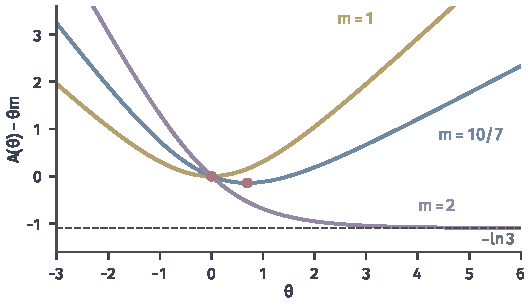
\includegraphics[width=90mm]{figures/07-probability/07-distribution-optimization/matplotlib/dsel-dual-function/figure.pdf}
 \caption{对偶函数取负号后的$A(\theta)-\theta m$，$A(\theta)=\ln\frac{1+\mathrm{e}^{\theta}+\mathrm{e}^{2\theta}}{3}$。黄：$m=1$，最小值$0$在$\theta=0$；蓝：$m=10/7$，最小值$-0.1429$在$\theta=\ln2$（红点）；紫：$m=2$，单调下降，下确界$-\ln3$（深灰虚线）不被达到。}
 \label{fig:dsel-dual-function}
\end{BookInlineFigure}

\paragraph{Hessian与局部求解}
对偶函数的Hessian是协方差矩阵的相反数。对任意$\bm{a}$，
\[
 \bm{a}^{\top}\operatorname{Cov}_{Q_{\bm{\theta}}}(\bm{T})\,\bm{a}=\operatorname{Var}_{Q_{\bm{\theta}}}\bigl(\langle\bm{a},\bm{T}\rangle\bigr)\geq0 ,
\]
等号当且仅当$\langle\bm{a},\bm{T}\rangle$在$Q_{\bm{\theta}}$下几乎必然为常数。有限状态、$p>0$时$Q_{\bm{\theta}}$处处为正，这就是$\langle\bm{a},\bm{T}(x)\rangle$对所有$x$相等。若不存在这样的$\bm{a}\neq\bm{0}$，即统计量之间没有仿射关系，则协方差矩阵对每个$\bm{\theta}$正定。

协方差正定时，$\bm{\theta}\mapsto\nabla A(\bm{\theta})$的Jacobian矩阵可逆，由反函数定理（见\BookChapterRef{chap:implicit-inverse-functions}{卷二第22章“隐函数与反函数”}），它的逆$\bm{m}\mapsto\bm{\theta}(\bm{m})$在$\operatorname{ri}\mathcal{M}$上光滑，导数是协方差矩阵的逆：
\[
 \frac{\partial\bm{\theta}}{\partial\bm{m}}=\operatorname{Cov}_{Q_{\bm{\theta}}}(\bm{T})^{-1} .
\]
在例子中$m=10/7$处$\operatorname{Var}_{Q_{\ln2}}(X)=26/49$，所以$\mathrm{d}\theta/\mathrm{d}m=49/26\approx1.885$：平均值再提高$0.01$，参数约需增加$0.019$。方差越小，同样的矩变化需要越大的参数变化；靠近可行矩集合的边界时方差趋于零，参数随之发散，这在后面的边界情形中会看到。

求解方程~\eqref{eq:dsel-moment-matching}的标准方法是Newton法：在当前点把$\nabla A$线性化，令线性化后的矩等于$\bm{m}$。迭代公式是
\begin{equation}
 \bm{\theta}^{(t+1)}=\bm{\theta}^{(t)}-\operatorname{Cov}_{Q_{\bm{\theta}^{(t)}}}(\bm{T})^{-1}\Bigl(\mathbb{E}_{Q_{\bm{\theta}^{(t)}}}[\bm{T}]-\bm{m}\Bigr).
 \label{eq:dsel-newton}
\end{equation}
它也是对凹函数$\ell$的Newton法（见\BookChapterRef{chap:second-order-methods}{卷五第7章“二阶方法”}）。每一步需要在当前倾斜分布下计算$\bm{T}$的均值与协方差。

在例子中从$\theta^{(0)}=0$出发。此时$Q$均匀，均值$1$，方差$2/3$，由式~\eqref{eq:dsel-newton}，
\[
 \theta^{(1)}=0-\frac{1-10/7}{2/3}=\frac{9}{14}\approx0.6429 .
\]
在$\theta^{(1)}$处，$Q\approx(0.1534,0.2917,0.5549)$，均值约$1.40147$，方差约$0.54708$，于是
\[
 \theta^{(2)}\approx0.6429-\frac{1.40147-1.42857}{0.54708}\approx0.692394 .
\]
再一步得到$\theta^{(3)}\approx0.6931470$，与$\ln2=0.69314718\ldots$相差约$2\times10^{-7}$。矩残差依次约为$0.43$、$2.7\times10^{-2}$、$4.0\times10^{-4}$、$9.4\times10^{-8}$，每步有效数字约翻倍，这是Newton法在解附近的二次收敛。

离解较远时，线性化可能越过头。图~\ref{fig:dsel-newton-steps}(a)从$\theta^{(0)}=-1$出发，第一步跳到$1.365$，越过了$\ln2$，第二步回到$0.451$，之后才进入二次收敛的范围。因为$\ell$是凹的，加上沿Newton方向的步长搜索即可保证从任意起点收敛；协方差接近奇异时，步长与方程的病态都要另作处理。

\begin{BookInlineFigure}
 \centering
 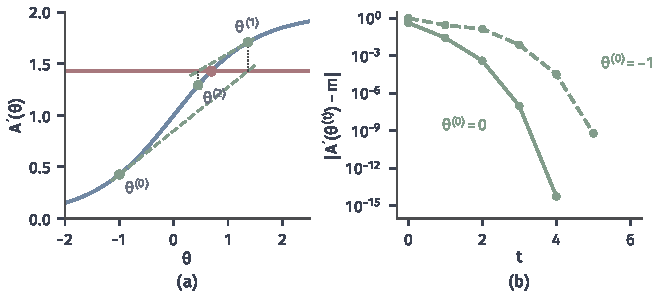
\includegraphics[width=112mm]{figures/07-probability/07-distribution-optimization/matplotlib/dsel-newton-steps/figure.pdf}
 \caption{用Newton法解矩匹配方程$A'(\theta)=10/7$。(a)均值映射$A'(\theta)$（蓝），目标水平$m=10/7$（红线），从$\theta^{(0)}=-1$出发的前两条切线（绿色虚线）与迭代点（绿）；红点是解$\theta=\ln2$。(b)矩残差$\lvert A'(\theta^{(t)})-m\rvert$，纵轴为对数刻度，实线从$\theta^{(0)}=0$出发，虚线从$\theta^{(0)}=-1$出发。}
 \label{fig:dsel-newton-steps}
\end{BookInlineFigure}

\paragraph{冗余统计量}
若统计量之间有仿射关系，协方差矩阵就奇异，Newton步中的线性方程不能唯一求解。取$\bm{T}(x)=(x,\,2-x)$，要求$\bm{m}=(\tfrac{10}7,\tfrac47)$。两个约束说的是同一件事，因为$T_1+T_2\equiv2$。倾斜分布为
\[
 q_{\bm{\theta}}(x)\propto\mathrm{e}^{\theta_1x+\theta_2(2-x)}=\mathrm{e}^{2\theta_2}\,\mathrm{e}^{(\theta_1-\theta_2)x},
\]
只依赖$\theta_1-\theta_2$。满足矩约束的$\bm{\theta}$组成整条直线$\theta_1-\theta_2=\ln2$，它们给出同一个$Q^{*}=(\tfrac17,\tfrac27,\tfrac47)$，正如定理~\ref{thm:dsel-min-kl}第三部分所说。记$v=\operatorname{Var}_{Q_{\bm{\theta}}}(X)$，协方差矩阵
\[
 \operatorname{Cov}_{Q_{\bm{\theta}}}(\bm{T})=v\begin{bmatrix}1&-1\\-1&1\end{bmatrix}
\]
沿$(1,1)$方向为零。图~\ref{fig:dsel-redundant}中，对偶函数的等值线都平行于$(1,1)$，最大值点不是一个点而是一条谷线。

\begin{BookInlineFigure}
 \centering
 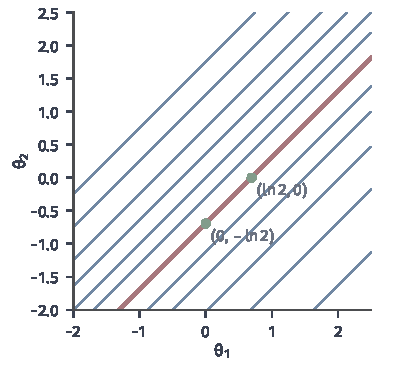
\includegraphics[width=70mm]{figures/07-probability/07-distribution-optimization/matplotlib/dsel-redundant/figure.pdf}
 \caption{冗余统计量$\bm{T}(x)=(x,2-x)$时的对偶函数，$P$均匀，$\bm{m}=(\frac{10}7,\frac47)$。蓝线是$A(\bm{\theta})-\langle\bm{\theta},\bm{m}\rangle$的等值线，全部平行于$(1,1)$；红线$\theta_1-\theta_2=\ln2$上每一点都是最优参数，绿点$(0,-\ln2)$与$(\ln2,0)$是其中两个，它们给出同一个分布。}
 \label{fig:dsel-redundant}
\end{BookInlineFigure}

处理办法有两种：删去多余的统计量，使表示成为第~\ref{chap:distribution-families}章的最小表示；或者保留冗余，在奇异的线性方程中取任意一个解，例如范数最小的解，最后得到的分布不受影响。冗余还带来一个必须先检查的问题：矩要求本身要相容。若要求$\bm{m}=(\tfrac{10}7,1)$，则$m_1+m_2\neq2$，$\bm{m}$不在$\operatorname{aff}\mathcal{M}$中，没有任何分布满足它；这时Newton迭代找不到解，问题出在约束而不在算法。

\paragraph{边界上的矩}
最后看$\bm{m}\in\mathcal{M}$但不在相对内部的情形。取$T(x)=\mathbf{1}_{\{x\geq1\}}$，$P$均匀，可行矩集合是$[0,1]$。对$0<m<1$，倾斜分布与矩约束为
\[
 Q_\theta=\frac{(1,\ \mathrm{e}^{\theta},\ \mathrm{e}^{\theta})}{1+2\mathrm{e}^{\theta}},\qquad\frac{2\mathrm{e}^{\theta}}{1+2\mathrm{e}^{\theta}}=m .
\]
解得$\theta(m)=\ln\dfrac{m}{2(1-m)}$，最优分布是$(1-m,\ \tfrac m2,\ \tfrac m2)$。

$m\to1$时$\theta(m)\to+\infty$。而$m=1$时可行的分布只有$(0,s,1-s)$，$0\leq s\leq1$，它们的KL是
\[
 D_{\mathrm{KL}}\bigl((0,s,1-s)\Vert P\bigr)=s\ln(3s)+(1-s)\ln\bigl(3(1-s)\bigr),
\]
在$s=\tfrac12$处最小，最优分布是$(0,\tfrac12,\tfrac12)$，最优值$\ln\tfrac32\approx0.4055$。它在状态$0$上的概率为零，不等于任何$Q_\theta$，却是$\theta\to\infty$时$Q_\theta$的极限。图~\ref{fig:dsel-boundary-face}画出参数的发散与最优值的连续：$D^{*}(m)$平稳地趋于$\ln\tfrac32$，$\theta(m)$却趋于无穷。

\begin{BookInlineFigure}
 \centering
 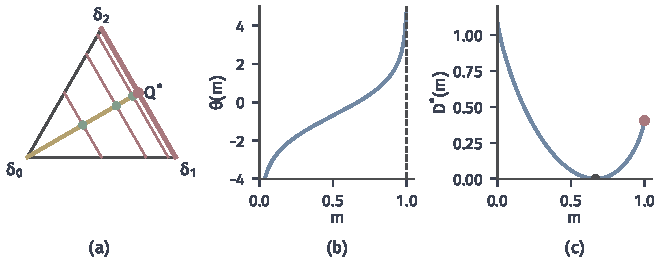
\includegraphics[width=112mm]{figures/07-probability/07-distribution-optimization/matplotlib/dsel-boundary-face/figure.pdf}
 \caption{边界上的矩，$T(x)=\mathbf{1}_{\{x\geq1\}}$，$P$均匀。(a)倾斜族是从$\delta_0$到$(0,\frac12,\frac12)$的线段（黄）；细红线是$m=0.5,0.8,0.95$的约束，绿点是各自的最优分布；粗红线是$m=1$时的可行集合，即$q(0)=0$的那条边，红点是最优分布。(b)参数$\theta(m)$，$m\to1$时发散。(c)最优值$D^{*}(m)$，在$m=2/3$处为零（$P$本身可行），在$m=1$处连续地达到$\ln\frac32$。}
 \label{fig:dsel-boundary-face}
\end{BookInlineFigure}

一般情形的结论如下。

\begin{theorem}[边界上的矩]
\label{thm:dsel-boundary}
设$\mathcal{X}$有限，$p(x)>0$对每个$x$成立，$\bm{m}\in\mathcal{M}\setminus\operatorname{ri}\mathcal{M}$。则
\begin{enumerate}
 \item 问题~\eqref{eq:dsel-min-kl-problem}有最优分布；
 \item 存在$\bm{a}\in\mathbb{R}^{k}$与$c\in\mathbb{R}$，使$\langle\bm{a},\bm{T}(x)\rangle\leq c$对一切$x$成立，$\langle\bm{a},\bm{m}\rangle=c$，且集合$F=\{x:\langle\bm{a},\bm{T}(x)\rangle=c\}$不是整个$\mathcal{X}$；每个$Q\in\mathcal{C}_{\bm{m}}$都满足$Q(F)=1$，因而没有任何$Q_{\bm{\theta}}$属于$\mathcal{C}_{\bm{m}}$；
 \item 对$Q(F)=1$的$Q$，记$P_F=P(\cdot\mid F)$，有
 \begin{equation}
 D_{\mathrm{KL}}(Q\Vert P)=D_{\mathrm{KL}}(Q\Vert P_F)-\ln P(F) ;
 \label{eq:dsel-face-reduction}
 \end{equation}
 \item 若$\bm{m}$属于$\operatorname{conv}\{\bm{T}(x):x\in F\}$的相对内部，则最优分布是$P_F$沿$\bm{T}$的倾斜$Q^{*}_F$，并且对满足$\mathbb{E}_{Q^{*}_F}[\bm{T}]=\bm{m}$的参数$\bm{\theta}_F$，$s\to+\infty$时$Q_{\bm{\theta}_F+s\bm{a}}\to Q^{*}_F$。
\end{enumerate}
\end{theorem}

\begin{proof}
第一部分。$\mathcal{C}_{\bm{m}}$由线性等式与非负性在概率单纯形中定出，是非空的有界闭集；$p>0$时$Q\mapsto\sum_xq(x)\ln(q(x)/p(x))$在单纯形上连续（约定$0\ln0=0$）。连续函数在非空紧集上取到最小值。

第二部分。$\mathcal{M}$是有限个点的凸包，$\bm{m}$在它的相对边界上。在仿射包$\operatorname{aff}\mathcal{M}$内对$\mathcal{M}$用凸集的支撑超平面定理，得到$\bm{a}\in L$（$L$是$\operatorname{aff}\mathcal{M}$的方向子空间）与$c$，使$\langle\bm{a},\bm{t}\rangle\leq c$对$\bm{t}\in\mathcal{M}$成立，$\langle\bm{a},\bm{m}\rangle=c$，且$\langle\bm{a},\cdot\rangle$在$\mathcal{M}$上不是常数。最后一点说明$F\neq\mathcal{X}$。对$Q\in\mathcal{C}_{\bm{m}}$，
\[
 \sum_xq(x)\bigl(c-\langle\bm{a},\bm{T}(x)\rangle\bigr)=c-\langle\bm{a},\bm{m}\rangle=0 .
\]
各项非负而和为零，所以$x\notin F$时$q(x)=0$，即$Q(F)=1$。每个$Q_{\bm{\theta}}$在所有状态上为正，不满足这一点。

第三部分。$x\in F$时$p_F(x)=p(x)/P(F)$，所以
\[
 \ln\frac{q(x)}{p(x)}=\ln\frac{q(x)}{p_F(x)}-\ln P(F) .
\]
乘以$q(x)$对$x\in F$求和，即得式~\eqref{eq:dsel-face-reduction}。所以在$F$上，原问题与以$P_F$为参考分布的同一问题只差常数$-\ln P(F)$。

第四部分。对状态集$F$、参考分布$P_F$与约束$\bm{m}$用定理~\ref{thm:dsel-min-kl}，得到最优分布$Q^{*}_F$与参数$\bm{\theta}_F$；由第三部分它也是原问题的最优分布。对$s>0$，
\[
 q_{\bm{\theta}_F+s\bm{a}}(x)\propto p(x)\,\mathrm{e}^{\langle\bm{\theta}_F,\bm{T}(x)\rangle}\,\mathrm{e}^{s(\langle\bm{a},\bm{T}(x)\rangle-c)} ,
\]
这里把各项同乘了与$x$无关的$\mathrm{e}^{-sc}$。$s\to\infty$时，最后一个因子在$F$上恒为$1$，在$F$外趋于$0$。归一化后的极限正比于$p(x)\mathrm{e}^{\langle\bm{\theta}_F,\bm{T}(x)\rangle}\mathbf{1}_F(x)$，这就是$Q^{*}_F$。
\end{proof}

若$\bm{m}$在$\operatorname{conv}\{\bm{T}(x):x\in F\}$中仍在相对边界上，对$F$重复第二、三部分，支持再缩小一次；状态有限，几步之内就会停下。在上面的例子中，$\bm{a}=1$，$c=1$，$F=\{1,2\}$，$T$在$F$上恒为$1$，$P_F=(0,\tfrac12,\tfrac12)$不需再倾斜，最优值$-\ln P(F)=\ln\tfrac32$。

边界情形说明了有限参数公式的局限。最优分布存在，也仍是某个倾斜的极限，但它收缩了支持，不能写成任何有限$\bm{\theta}$的$Q_{\bm{\theta}}$。数值上，Newton迭代的$\bm{\theta}$会越走越远：在$T(x)=x$、$m=2$的例子中，参数每步大约增加$1$，残差每步只缩小到约$1/\mathrm{e}$，内部情形的二次收敛不复存在。遇到这种迹象，应当先识别哪些状态的概率必须为零，在缩小后的状态集上重新求解，而不是继续追逐发散的参数。对偶函数的上确界仍等于最优值，沿$\bm{\theta}_F+s\bm{a}$可以逼近，只是取不到。


\section{最大熵}
\label{sec:dsel-maxent}

一颗骰子，我们只知道长期掷出的平均点数是$4.5$，此外一无所知。若要给出一张概率表，该用哪一张？满足平均点数$4.5$的表有无穷多张。若选了一张让$6$点特别多、$1$点为零的表，就等于声称知道了“$1$点不会出现”之类平均值并未告诉我们的事。一个自然的原则是：在满足已知条件的分布中，选最不确定的那个，也就是熵最大的那个。

第~\ref{chap:information-measures}章把熵$H(Q)=-\sum_xq(x)\ln q(x)$解释为平均要问的是非题数目（以nat计）。熵越大，结果越难预测，分布中隐含的额外断言就越少。按这个标准选择分布，称为\term{最大熵原理}（maximum entropy principle）。它是一条选择规则，不是定理；定理要回答的是，按这条规则选出的分布是什么、何时存在。

\paragraph{有限支持上的最大熵}
设$\mathcal{X}$有$n$个状态，$U$是$\mathcal{X}$上的均匀分布。对$\mathcal{X}$上任意分布$Q$，
\[
 D_{\mathrm{KL}}(Q\Vert U)=\sum_xq(x)\ln\bigl(n\,q(x)\bigr)=\ln n-H(Q) .
\]
所以
\begin{equation}
 H(Q)=\ln n-D_{\mathrm{KL}}(Q\Vert U).
 \label{eq:dsel-entropy-kl-uniform}
\end{equation}
熵与“离均匀分布的KL”只差一个与$Q$无关的常数，最大化熵就是以均匀分布为参考、最小化KL。上一节的结论可以直接搬过来。

\begin{theorem}[有限支持上的最大熵分布]
\label{thm:dsel-maxent-finite}
设$\mathcal{X}$有限，$\bm{T}:\mathcal{X}\to\mathbb{R}^{k}$，$\bm{m}\in\operatorname{ri}\operatorname{conv}\{\bm{T}(x):x\in\mathcal{X}\}$。则在$\mathbb{E}_{Q}[\bm{T}]=\bm{m}$的分布中，熵的最大值由唯一的分布
\begin{equation}
 q^{*}(x)=\frac{\exp\langle\bm{\theta},\bm{T}(x)\rangle}{\sum_{y\in\mathcal{X}}\exp\langle\bm{\theta},\bm{T}(y)\rangle}
 \label{eq:dsel-maxent-finite}
\end{equation}
达到，其中$\bm{\theta}$满足$\mathbb{E}_{Q^{*}}[\bm{T}]=\bm{m}$。最大熵为
\begin{equation}
 H(Q^{*})=A_0(\bm{\theta})-\langle\bm{\theta},\bm{m}\rangle,\qquad A_0(\bm{\theta})=\ln\sum_{y\in\mathcal{X}}\mathrm{e}^{\langle\bm{\theta},\bm{T}(y)\rangle} .
 \label{eq:dsel-maxent-value}
\end{equation}
\end{theorem}

\begin{proof}
由式~\eqref{eq:dsel-entropy-kl-uniform}，问题等价于以$P=U$为参考的问题~\eqref{eq:dsel-min-kl-problem}。$U$处处为正，定理~\ref{thm:dsel-min-kl}给出唯一最优分布
\[
 q^{*}(x)=\frac1n\exp\bigl(\langle\bm{\theta},\bm{T}(x)\rangle-A(\bm{\theta})\bigr),
\]
其中
\[
 A(\bm{\theta})=\ln\frac1n\sum_y\mathrm{e}^{\langle\bm{\theta},\bm{T}(y)\rangle}=A_0(\bm{\theta})-\ln n ,
\]
代入即得式~\eqref{eq:dsel-maxent-finite}。最大熵等于$\ln n-D^{*}$，由式~\eqref{eq:dsel-min-kl-value}，
\[
 H(Q^{*})=\ln n-\langle\bm{\theta},\bm{m}\rangle+A_0(\bm{\theta})-\ln n=A_0(\bm{\theta})-\langle\bm{\theta},\bm{m}\rangle .
\]
\end{proof}

式~\eqref{eq:dsel-maxent-finite}称为\term{最大熵分布}（maximum entropy distribution）。定理中的“支持”是事先给定的：状态集合$\mathcal{X}$本身就是一条约束，不在其中的状态概率为零。若把骰子的状态集合扩大到$\{0,1,\dots,7\}$，$\ln n$和最大熵分布都会改变。在有限情形中，计数测度把每个状态看成同样重要，这是“均匀分布最不确定”的前提。

在三状态的例子中，均值$10/7$下的最大熵分布就是$(\tfrac17,\tfrac27,\tfrac47)$，熵为
\[
 H(Q^{*})=\ln7-\frac{10}{7}\ln2\approx0.9557 .
\]
约束线段的端点$(\tfrac27,0,\tfrac57)$的熵约为$0.5983$。由式~\eqref{eq:dsel-entropy-kl-uniform}与勾股恒等式，两者之差恰为$D_{\mathrm{KL}}(Q\Vert Q^{*})\approx0.3574$：熵的损失就是离最大熵分布的KL。

\paragraph{约束改变时}
回到骰子，$\mathcal{X}=\{1,\dots,6\}$，$T(x)=x$，可行矩集合是$[1,6]$。均值$m$给定后，最大熵分布是$q(x)\propto\mathrm{e}^{\theta x}$，$\theta$由
\[
 \frac{\sum_{x=1}^{6}x\,\mathrm{e}^{\theta x}}{\sum_{x=1}^{6}\mathrm{e}^{\theta x}}=m
\]
确定。它没有闭式解，用第~\ref{sec:dsel-moment-matching}节的Newton法求出。

$m=3.5$时，均匀分布本身满足约束，$\theta=0$，熵为$\ln6\approx1.792$。约束没有起作用：它排除了一些分布，但没有排除熵最大的那个。$m=4.5$时，$\theta\approx0.3710$，
\[
 Q^{*}\approx(0.0544,\ 0.0788,\ 0.1142,\ 0.1654,\ 0.2398,\ 0.3475),
\]
熵约为$1.614$。相邻点数的概率之比恒为$\mathrm{e}^{\theta}\approx1.449$，平均值的要求以最平缓的方式把质量推向大点数，没有任何一面被删去。$m=5.5$时$\theta\approx1.087$，分布约为$(0.0029,0.0086,0.0255,0.0755,0.2238,0.6637)$，熵降到约$0.953$。

再加一条约束。要求均值为$3.5$，且$\mathbb{E}_{Q}[(X-3.5)^{2}]=1$，比均匀分布的$35/12\approx2.917$小。统计量取$\bm{T}(x)=\bigl(x-3.5,\ (x-3.5)^{2}\bigr)$，由对称性第一个乘子为零，最大熵分布是$q(x)\propto\mathrm{e}^{\theta_2(x-3.5)^{2}}$，$\theta_2\approx-0.4887$：
\[
 Q^{*}\approx(0.0186,\ 0.1316,\ 0.3498,\ 0.3498,\ 0.1316,\ 0.0186),
\]
熵约为$1.417$。它是一个离散的钟形，这正是指数中出现二次项的结果。图~\ref{fig:dsel-dice-bars}画出这四张表。

\begin{BookInlineFigure}
 \centering
 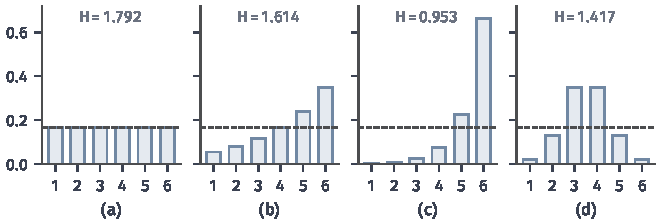
\includegraphics[width=112mm]{figures/07-probability/07-distribution-optimization/matplotlib/dsel-dice-bars/figure.pdf}
 \caption{骰子的最大熵分布（蓝色柱），深灰虚线为均匀概率$1/6$，图中标出熵（nat）。(a)$\mathbb{E}[X]=3.5$，约束不起作用。(b)$\mathbb{E}[X]=4.5$，$\theta\approx0.371$。(c)$\mathbb{E}[X]=5.5$，$\theta\approx1.087$。(d)$\mathbb{E}[X]=3.5$且$\mathbb{E}[(X-3.5)^{2}]=1$，$q\propto\mathrm{e}^{\theta_2(x-3.5)^{2}}$，$\theta_2\approx-0.489$。}
 \label{fig:dsel-dice-bars}
\end{BookInlineFigure}

增加约束只会缩小可行集合，最大熵不会增加；(d)比(a)少了约$0.375$ nat，这就是“方差为$1$”这条信息的量。最大熵还随约束值连续变化。记$H^{*}(m)$为均值为$m$时的最大熵。设$Q_1,Q_2$分别是均值$m_1,m_2$下的最大熵分布，$0\leq\lambda\leq1$，混合$\lambda Q_1+(1-\lambda)Q_2$的均值是$\lambda m_1+(1-\lambda)m_2$，由熵的凹性，
\[
 H^{*}\bigl(\lambda m_1+(1-\lambda)m_2\bigr)\geq H\bigl(\lambda Q_1+(1-\lambda)Q_2\bigr)\geq\lambda H^{*}(m_1)+(1-\lambda)H^{*}(m_2) .
\]
所以$H^{*}$是凹函数。图~\ref{fig:dsel-entropy-curve}(a)中它在$m=3.5$处取最大值$\ln6$，向两端下降，在$m=1$和$m=6$处为零，那里唯一可行的分布是单点分布；(b)中的$\theta(m)$在两端发散，与第~\ref{sec:dsel-moment-matching}节的边界情形一致。

\begin{BookInlineFigure}
 \centering
 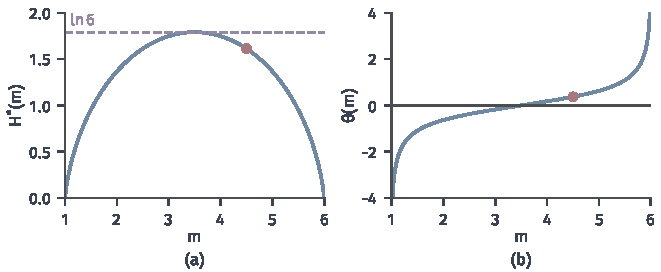
\includegraphics[width=112mm]{figures/07-probability/07-distribution-optimization/matplotlib/dsel-entropy-curve/figure.pdf}
 \caption{骰子均值为$m$时的最大熵问题。(a)最大熵$H^{*}(m)$（蓝），紫色虚线为上界$\ln6$，红点为$m=4.5$，$H^{*}\approx1.614$。(b)对应的乘子$\theta(m)$，红点为$(4.5,\,0.371)$，$m\to1$或$6$时发散。}
 \label{fig:dsel-entropy-curve}
\end{BookInlineFigure}

\paragraph{连续情形的参考测度}
对有密度的分布，第~\ref{chap:information-measures}章用微分熵$h=-\int f\ln f\,\mathrm{d}x$代替熵。这里的密度是相对于Lebesgue测度的密度，Lebesgue测度在其中扮演的角色，正是有限情形中的计数测度。一般地，设$\nu$是$\mathcal{X}$上的$\sigma$有限测度，$Q\ll\nu$，$q=\mathrm{d}Q/\mathrm{d}\nu$，在$q\lvert\ln q\rvert$对$\nu$可积时定义
\begin{equation}
 h_\nu(Q)=-\int_{\mathcal{X}}q\ln q\,\mathrm{d}\nu .
 \label{eq:dsel-entropy-reference}
\end{equation}
换一个参考测度，这个量就变成另一个泛函，最大化它得到的分布也随之不同。

看一个不带任何矩约束的例子：$\mathcal{X}=[1,\mathrm{e}]$。以$\nu=\mathrm{d}x$为参考，$\nu$的总质量是$\mathrm{e}-1$，记$R$为$[1,\mathrm{e}]$上的均匀分布，与式~\eqref{eq:dsel-entropy-kl-uniform}同样计算得
\[
 h_{\mathrm{d}x}(Q)=\ln(\mathrm{e}-1)-D_{\mathrm{KL}}(Q\Vert R),
\]
最大熵分布是均匀分布，密度$1/(\mathrm{e}-1)$。以$\nu(\mathrm{d}x)=\mathrm{d}x/x$为参考，总质量$\int_1^{\mathrm{e}}x^{-1}\,\mathrm{d}x=1$，$\nu$本身就是概率测度，
\[
 h_{\mathrm{d}x/x}(Q)=-D_{\mathrm{KL}}(Q\Vert\nu),
\]
最大熵分布是$\nu$本身，相对$\mathrm{d}x$的密度为$1/x$。换成变量$y=\ln x$，第二个参考测度就是$[0,1]$上的Lebesgue测度，它说的是“$\ln X$均匀”。两个答案的中位数分别是$(1+\mathrm{e})/2\approx1.859$与$\sqrt{\mathrm{e}}\approx1.649$，见图~\ref{fig:dsel-reference-measure}。同样是“一无所知”，用$x$计量还是用$\ln x$计量，给出不同的分布。

\begin{BookInlineFigure}
 \centering
 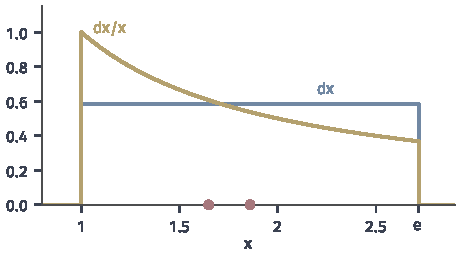
\includegraphics[width=78mm]{figures/07-probability/07-distribution-optimization/matplotlib/dsel-reference-measure/figure.pdf}
 \caption{参考测度决定最大熵分布，$\mathcal{X}=[1,\mathrm{e}]$，无矩约束。蓝：以$\mathrm{d}x$为参考，得到均匀密度$1/(\mathrm{e}-1)$；黄：以$\mathrm{d}x/x$为参考，得到密度$1/x$，即$\ln X$在$[0,1]$上均匀。两个红点是二者的中位数$\sqrt{\mathrm{e}}$与$(1+\mathrm{e})/2$。}
 \label{fig:dsel-reference-measure}
\end{BookInlineFigure}

所以在连续情形中谈最大熵，必须先说明熵是相对哪个测度计算的。有限情形中这个问题被状态集合的选择掩盖了：一旦把骰子的六面当作六个状态，计数测度就是默认的参考。

\paragraph{熵与KL的差别}
在有限情形中，最大熵与以均匀分布为参考的最小KL只差常数。一般的参考概率$P$却不能这样替换。设$P$相对$\nu$的密度$p$处处为正，$Q$相对$\nu$的密度为$q$。在$\{q>0\}$上把$\ln q$拆成$\ln(q/p)+\ln p$，乘以$q$积分，在两项都有限时得到
\begin{equation}
 h_\nu(Q)=-D_{\mathrm{KL}}(Q\Vert P)-\mathbb{E}_{Q}[\ln p] .
 \label{eq:dsel-entropy-kl-reference}
\end{equation}
第二项依赖于$Q$，所以最大化$h_\nu$与最小化$D_{\mathrm{KL}}(\cdot\Vert P)$一般选出不同的分布。负熵$-h_\nu$是“相对于$\nu$”的KL，而不是相对于某个概率分布的KL；在有限情形中两者相同，只因为$\ln p$是常数$-\ln n$。

第二项在可行集合上为常数的情形是例外。若$\ln p$是约束统计量的仿射函数，
\[
 \ln p=\langle\bm{\theta},\bm{T}\rangle-A(\bm{\theta}),
\]
则对每个满足$\mathbb{E}_{Q}[\bm{T}]=\bm{m}$的$Q$，$\mathbb{E}_{Q}[\ln p]$都等于同一个常数$\langle\bm{\theta},\bm{m}\rangle-A(\bm{\theta})$，最大熵与最小KL就重合了。下面的定理正是这样证明的。

\begin{theorem}[相对参考测度的最大熵]
\label{thm:dsel-maxent-continuous}
设$\nu$是$\mathcal{X}$上的$\sigma$有限测度，$\bm{T}:\mathcal{X}\to\mathbb{R}^{k}$可测。设$\bm{\theta}$使
\begin{equation}
 A(\bm{\theta})=\ln\int_{\mathcal{X}}\mathrm{e}^{\langle\bm{\theta},\bm{T}\rangle}\,\mathrm{d}\nu<\infty ,
 \label{eq:dsel-maxent-partition}
\end{equation}
并且相对$\nu$的密度为
\begin{equation}
 q_{\bm{\theta}}=\exp\bigl(\langle\bm{\theta},\bm{T}\rangle-A(\bm{\theta})\bigr)
 \label{eq:dsel-maxent-density}
\end{equation}
的分布$Q_{\bm{\theta}}$满足$\mathbb{E}_{Q_{\bm{\theta}}}\lVert\bm{T}\rVert_2<\infty$，$\mathbb{E}_{Q_{\bm{\theta}}}[\bm{T}]=\bm{m}$。则对每个满足$Q\ll\nu$、$q\lvert\ln q\rvert$对$\nu$可积、$\mathbb{E}_{Q}\lVert\bm{T}\rVert_2<\infty$且$\mathbb{E}_{Q}[\bm{T}]=\bm{m}$的分布$Q$，
\begin{equation}
 h_\nu(Q)=h_\nu(Q_{\bm{\theta}})-D_{\mathrm{KL}}(Q\Vert Q_{\bm{\theta}}),\qquad h_\nu(Q_{\bm{\theta}})=A(\bm{\theta})-\langle\bm{\theta},\bm{m}\rangle .
 \label{eq:dsel-maxent-identity}
\end{equation}
因此$Q_{\bm{\theta}}$是这些分布中熵最大的唯一一个。
\end{theorem}

\begin{proof}
$q_{\bm{\theta}}$处处为正，所以$Q\ll Q_{\bm{\theta}}$，密度比为$q/q_{\bm{\theta}}$。在$\{q>0\}$上，
\[
 \ln\frac{q}{q_{\bm{\theta}}}=\ln q-\langle\bm{\theta},\bm{T}\rangle+A(\bm{\theta}) .
\]
右边三项都在$Q$下可积：$\int q\lvert\ln q\rvert\,\mathrm{d}\nu<\infty$，$\bm{T}$在$Q$下可积，$A(\bm{\theta})$是常数。逐项取$Q$下的期望，
\[
 D_{\mathrm{KL}}(Q\Vert Q_{\bm{\theta}})=-h_\nu(Q)-\langle\bm{\theta},\bm{m}\rangle+A(\bm{\theta}) .
\]
对$Q=Q_{\bm{\theta}}$，由
\[
 \lvert\ln q_{\bm{\theta}}\rvert\leq\lvert\langle\bm{\theta},\bm{T}\rangle\rvert+\lvert A(\bm{\theta})\rvert
\]
知$\ln q_{\bm{\theta}}$在$Q_{\bm{\theta}}$下可积，它满足同样的条件，代入上式，左边为零，得到式~\eqref{eq:dsel-maxent-identity}的第二式。把第二式代回上式，就得到第一式。唯一性来自Gibbs不等式的等号条件。
\end{proof}

定理的形式与有限情形相同，不同之处在于两件事都要事先核对：配分积分$\int\mathrm{e}^{\langle\bm{\theta},\bm{T}\rangle}\mathrm{d}\nu$是否有限，以及候选分布的熵是否有定义。第~\ref{chap:information-measures}章已经指出，密度可以大于$1$，$-q\ln q$有正有负，正负两部分的积分都发散时熵没有意义；这样的分布不在定理比较的范围内。

\paragraph{几个连续例子}
在$\mathbb{R}$上以Lebesgue测度为参考，规定均值$\mu$与方差$\sigma^{2}$，即$\bm{T}(x)=(x,x^{2})$，$\bm{m}=(\mu,\mu^{2}+\sigma^{2})$。候选形式是$\mathrm{e}^{\theta_1x+\theta_2x^{2}}$，可积要求$\theta_2<0$，它就是高斯密度；$\mathcal{N}(\mu,\sigma^{2})$满足约束，由定理~\ref{thm:dsel-maxent-continuous}，它是给定均值与方差的密度中微分熵最大的，最大值为
\[
 h\bigl(\mathcal{N}(\mu,\sigma^{2})\bigr)=\frac12\ln(2\pi\mathrm{e}\sigma^{2}) .
\]
方差为$1$时它约为$1.419$。同样方差为$1$的Laplace密度微分熵约为$1.347$，$[-\sqrt3,\sqrt3]$上的均匀密度约为$1.242$，都更小，见图~\ref{fig:dsel-gauss-maxent}。

\begin{BookInlineFigure}
 \centering
 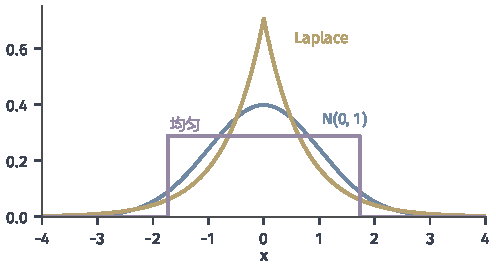
\includegraphics[width=84mm]{figures/07-probability/07-distribution-optimization/matplotlib/dsel-gauss-maxent/figure.pdf}
 \caption{均值$0$、方差$1$的三个密度。蓝：$\mathcal{N}(0,1)$，$h=\frac12\ln(2\pi\mathrm{e})\approx1.419$；黄：尺度$1/\sqrt2$的Laplace密度，$h=1+\ln\sqrt2\approx1.347$；紫：$[-\sqrt3,\sqrt3]$上的均匀密度，$h=\ln(2\sqrt3)\approx1.242$。熵相对Lebesgue测度计算，单位为nat。}
 \label{fig:dsel-gauss-maxent}
\end{BookInlineFigure}

在$(0,\infty)$上规定均值$1/\lambda$，候选$\mathrm{e}^{\theta x}$要求$\theta<0$，得到$\operatorname{Exp}(\lambda)$，最大熵为$1-\ln\lambda$。在有界区间$[a,b]$上不加任何矩约束，$\bm{T}=\bm{0}$，得到均匀分布，最大熵为$\ln(b-a)$。这三个常见分布都是“在某个支持上、给定某些矩”时的最大熵分布，支持与矩缺一不可。

最大值也可能不存在。在$\mathbb{R}$上只规定均值$\mu$，候选形式$\mathrm{e}^{\theta x}$对任何$\theta$都不可积，定理无从适用；而$\mathcal{N}(\mu,s^{2})$都满足约束，熵$\frac12\ln(2\pi\mathrm{e}s^{2})$随$s\to\infty$趋于无穷，所以上确界是$+\infty$。在$(0,\infty)$上不加约束也是如此。Lebesgue测度的总质量无穷，质量可以无限摊开，熵就没有上界。


\section{解的检验}
\label{sec:dsel-checks}

前三节都先用乘子或驻点“猜”出解的形式，再用一个恒等式验证它。实际计算中，候选分布还可能来自截断的级数、数值迭代或随机估计，它未必满足原问题的全部要求。拿到一个候选$\widehat{Q}$后，应当回到原问题依次回答三个问题：它是不是合法的候选，最小值存不存在，它是否达到了最小值或离最小值还有多远。图~\ref{fig:dsel-check-flow}把这些检查排成一条链。

\begin{BookInlineFigure}
 \centering
 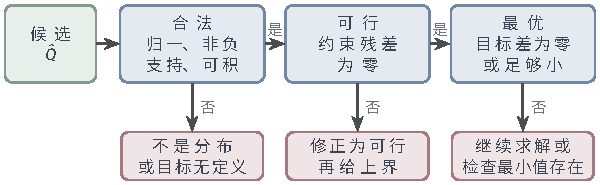
\includegraphics[width=102mm]{figures/07-probability/07-distribution-optimization/tikz/dsel-check-flow/figure.pdf}
 \caption{候选分布的检查顺序。绿框是待检的候选，蓝框是依次要通过的检查，红框是未通过时的处理：不合法的候选不能参加比较；不满足约束的候选先修正为可行分布，再用于给出最优值的上界；目标差不够小时继续求解，或回头检查最小值是否存在。}
 \label{fig:dsel-check-flow}
\end{BookInlineFigure}

\paragraph{候选是否合法}
第一步核对第~\ref{sec:dsel-problems}节列出的各项。归一化与非负性：指数形式的公式保证非负，但若配分函数是截断级数或数值积分得到的，归一化可能只是近似成立。支持：所有候选都要满足$\widehat{Q}\ll P$；倾斜公式自动满足，边界解则需要明确哪些状态的概率为零。可积性：目标与约束中的期望都要有限，下面会看到一个写得出公式、却因可积性失败而不合法的例子。

约束问题还要检查约束残差$\bm{r}=\mathbb{E}_{\widehat{Q}}[\bm{T}]-\bm{m}$。以第~\ref{sec:dsel-moment-matching}节Newton法的第一步为例，$\theta^{(1)}=9/14$给出
\[
 \widehat{Q}=Q_{\theta^{(1)}}\approx(0.1534,\ 0.2917,\ 0.5549),\qquad r\approx1.40147-1.42857=-0.0271 .
\]
它不满足约束，不属于可行集合。这时它的KL值$D_{\mathrm{KL}}(\widehat{Q}\Vert P)\approx0.1248$比真正的最优值$0.1429$还小，若把它当作“最小KL”报告就错了：违反约束的候选可以比最优解更好。

\paragraph{目标差}
不可行的倾斜分布并非没有用处。式~\eqref{eq:dsel-weak-duality}说明，任何$\bm{\theta}$都给出最优值的下界$\ell(\bm{\theta})$；再把$\widehat{Q}$修正成一个可行分布$\widetilde{Q}$，就得到上界$D_{\mathrm{KL}}(\widetilde{Q}\Vert P)$。两者之差
\begin{equation}
 D_{\mathrm{KL}}(\widetilde{Q}\Vert P)-\ell(\bm{\theta})\geq D_{\mathrm{KL}}(\widetilde{Q}\Vert P)-D^{*}\geq0
 \label{eq:dsel-certificate}
\end{equation}
控制了$\widetilde{Q}$离最优还差多少，这就是\term{最优性证书}（optimality certificate）：不必知道$D^{*}$，就能保证误差不超过一个算得出的数。

在例子中，$\widehat{Q}$的均值偏小，把它与均值最大的点质量$\delta_2$混合：
\[
 \widetilde{Q}=(1-\alpha)\widehat{Q}+\alpha\delta_2 ,
\]
均值为$(1-\alpha)\cdot1.40147+2\alpha$。令它等于$10/7$，解得
\[
 \alpha=\frac{10/7-1.40147}{2-1.40147}\approx0.04528 .
\]
修正后的$\widetilde{Q}\approx(0.1464,0.2785,0.5750)$可行，上界与下界分别为
\[
 D_{\mathrm{KL}}(\widetilde{Q}\Vert P)\approx0.143059,\qquad\ell(\theta^{(1)})=\frac{10}{7}\cdot\frac{9}{14}-A\Bigl(\frac9{14}\Bigr)\approx0.142234 .
\]
两者相差约$8.3\times10^{-4}$，所以$\widetilde{Q}$的KL离最优值不超过$8.3\times10^{-4}$，而最优值被夹在$[0.142234,\ 0.143059]$中。

对后续的Newton迭代点做同样的事，得到表~\ref{tab:dsel-certificate}与图~\ref{fig:dsel-certificate}。第二步之后证书已小于$2\times10^{-7}$，第三步约为$10^{-14}$，与数值舍入相当。

\begin{BookInlineTable}
 \centering
 \caption{Newton迭代点的最优性证书，$P$均匀，$T(x)=x$，$m=10/7$，精确最优值$D^{*}\approx0.1429124$。$\alpha$是为满足约束而混入$\delta_2$的比例。}
 \label{tab:dsel-certificate}
 \begin{tabular}{ccccc}
 \toprule
 $t$ & $\theta^{(t)}$ & 下界$\ell(\theta^{(t)})$ & 上界$D_{\mathrm{KL}}(\widetilde{Q}\Vert P)$ & 证书 \\
 \midrule
 $0$ & $0$ & $0$ & $0.170028$ & $1.7\times10^{-1}$ \\
 $1$ & $0.642857$ & $0.142234$ & $0.143059$ & $8.3\times10^{-4}$ \\
 $2$ & $0.692394$ & $0.1429122$ & $0.1429124$ & $1.8\times10^{-7}$ \\
 $3$ & $0.693147$ & $0.1429124$ & $0.1429124$ & $1.0\times10^{-14}$ \\
 \bottomrule
 \end{tabular}
\end{BookInlineTable}

\begin{BookInlineFigure}
 \centering
 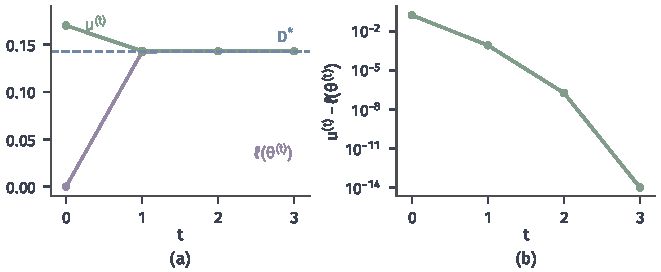
\includegraphics[width=112mm]{figures/07-probability/07-distribution-optimization/matplotlib/dsel-certificate/figure.pdf}
 \caption{最优性证书随Newton迭代的变化。(a)下界$\ell(\theta^{(t)})$（紫）与修正后可行分布的上界$u^{(t)}=D_{\mathrm{KL}}(\widetilde{Q}\Vert P)$（绿），蓝色虚线是$D^{*}$。(b)证书$u^{(t)}-\ell(\theta^{(t)})$，纵轴为对数刻度。}
 \label{fig:dsel-certificate}
\end{BookInlineFigure}

证书的两部分各有含义。在式~\eqref{eq:dsel-pythagoras-general}中分别取$Q=\widetilde{Q}$与$Q=Q^{*}$，得到
\[
 D_{\mathrm{KL}}(\widetilde{Q}\Vert P)-D^{*}=D_{\mathrm{KL}}(\widetilde{Q}\Vert Q^{*}),\qquad D^{*}-\ell(\bm{\theta})=D_{\mathrm{KL}}(Q^{*}\Vert Q_{\bm{\theta}}) .
\]
上界的误差是可行候选离最优分布的KL，下界的误差是最优分布离当前倾斜分布的KL。在第一步，两者约为$1.5\times10^{-4}$与$6.8\times10^{-4}$，和正是表中的$8.3\times10^{-4}$。

KL正则化的成本问题更直接。若$Z$能算出，最优值就是$-\tau\ln Z$，由式~\eqref{eq:dsel-gibbs-identity}，任何候选的目标差恰为$\tau D_{\mathrm{KL}}(\widehat{Q}\Vert Q^{*})$，不需要另找下界。

\paragraph{最小值是否存在}
有限状态上，可行集合非空时它是概率单纯形中的有界闭集，目标若在其上连续，最小值必然取到；第~\ref{sec:dsel-moment-matching}节的边界定理就是这样证明的。状态无穷时，这个论证会失效。

取$\mathcal{X}=\{1,2,\dots\}$，$P(k)=c/k^{3}$，$c=1/\sum_kk^{-3}\approx0.8319$。$P$的均值有限，
\[
 \mu=\mathbb{E}_{P}[X]=c\sum_{k\geq1}\frac1{k^{2}}=\frac{c\,\pi^{2}}{6}\approx1.3684 .
\]
要求$\mathbb{E}_{Q}[X]=2$，在可行分布中最小化$D_{\mathrm{KL}}(Q\Vert P)$。

先试倾斜。$q_\theta(k)\propto\mathrm{e}^{\theta k}/k^{3}$，当$\theta>0$时级数发散，倾斜分布不存在；当$\theta\leq0$时倾斜分布存在，但均值关于$\theta$不减（导数是方差），所以均值不超过$\theta=0$时的$\mu<2$。没有任何倾斜分布满足约束。

再看最优值。令$Q_N=(1-\varepsilon)P+\varepsilon\delta_N$，其中$\varepsilon=(2-\mu)/(N-\mu)$，它的均值是$\mu+\varepsilon(N-\mu)=2$，可行。$Q_N$与$P$的密度比在$k\neq N$处是$1-\varepsilon$，在$k=N$处是$1-\varepsilon+\varepsilon/P(N)$，所以
\[
 D_{\mathrm{KL}}(Q_N\Vert P)=(1-\varepsilon)\bigl(1-P(N)\bigr)\ln(1-\varepsilon)+Q_N(N)\ln\Bigl(1-\varepsilon+\frac{\varepsilon N^{3}}{c}\Bigr).
\]
第一项趋于零。第二项中$Q_N(N)\leq P(N)+\varepsilon$约为$0.632/N$，对数约为$2\ln N$，乘积约为$1.26\ln N/N$，也趋于零。数值上，$N=10,100,1000,10^{4}$时KL分别约为$0.261$、$0.0509$、$0.00793$、$0.00108$。所以最优值是$0$。

但最优值$0$达不到：$D_{\mathrm{KL}}(Q\Vert P)=0$只对$Q=P$成立，而$P$的均值是$1.3684$，不是$2$。图~\ref{fig:dsel-heavy-tail}画出这个机制：把极小的质量放到很远的地方，均值就能提高很多，KL的代价却微不足道。$Q_N$与$P$的总变差是$\varepsilon(1-P(N))\to0$，可是均值始终是$2$；函数$x$无界，均值不随分布的这种接近而连续变化，可行集合在这种收敛下不是闭的。

\begin{BookInlineFigure}
 \centering
 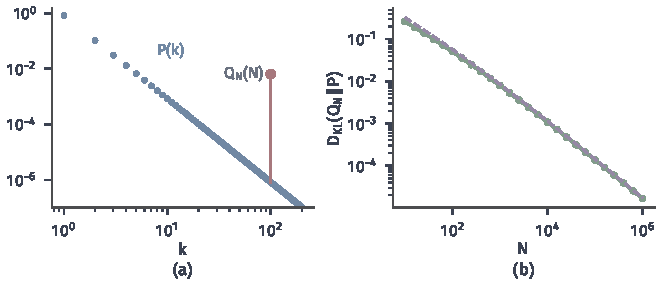
\includegraphics[width=112mm]{figures/07-probability/07-distribution-optimization/matplotlib/dsel-heavy-tail/figure.pdf}
 \caption{最小KL达不到的例子。$P(k)=c/k^{3}$，约束$\mathbb{E}_{Q}[X]=2$。(a)$P$的质量（蓝点），双对数坐标；$Q_{100}$把每项乘以$1-\varepsilon$，并在$k=100$处加上质量$\varepsilon\approx0.0064$（红）。(b)$D_{\mathrm{KL}}(Q_N\Vert P)$（绿）随$N$趋于零，紫色虚线是近似$\varepsilon\ln(\varepsilon N^{3}/c)$。}
 \label{fig:dsel-heavy-tail}
\end{BookInlineFigure}

一般空间中的存在性需要两方面的条件。一方面，KL的下水平集$\{Q:D_{\mathrm{KL}}(Q\Vert P)\leq a\}$在分布的弱收敛下是紧的，并且$D_{\mathrm{KL}}(\cdot\Vert P)$下半连续；证明需要用到下半连续函数的变分表示和第~\ref{chap:weak-convergence-of-distributions}章的胎紧性，可查阅~\scite{math-kallenberg2021probability}。另一方面，约束集合要在弱收敛下闭，例如$\bm{T}$有界连续时就是如此。两者都成立、且可行集合中有KL有限的分布时，最小值能取到。上面的例子缺的是第二条。

\paragraph{给出的分布是否达到最小值}
即使最优值有限、公式也写得出来，写出的分布仍可能不是候选。回到KL正则化的成本问题，取$\mathcal{X}=\{1,2,\dots\}$，$\tau=1$，
\[
 P(k)=c'\,\frac{\mathrm{e}^{-k}}{k^{2}},\qquad V(k)=-k ,
\]
其中$c'=1/\sum_k\mathrm{e}^{-k}k^{-2}\approx2.4465$。配分函数是
\[
 Z=\sum_{k\geq1}c'\frac{\mathrm{e}^{-k}}{k^{2}}\mathrm{e}^{k}=c'\frac{\pi^{2}}{6}\approx4.024 ,
\]
有限，Gibbs分布$Q^{*}(k)=\frac{6}{\pi^{2}k^{2}}$存在。可是
\[
 \mathbb{E}_{Q^{*}}\lvert V\rvert=\frac{6}{\pi^{2}}\sum_{k\geq1}\frac1k=\infty ,
\]
$Q^{*}$不在候选集合$\mathcal{Q}_V$中，定理~\ref{thm:dsel-gibbs-variational}的第二部分不适用。

第一部分仍然成立：对每个$Q\in\mathcal{Q}_V$，
\[
 J_1(Q)=-\ln Z+D_{\mathrm{KL}}(Q\Vert Q^{*})>-\ln Z ,
\]
严格不等号是因为$Q\neq Q^{*}$。另一方面，截断$Q_N=Q^{*}(\cdot\mid k\leq N)$只有有限个状态，属于$\mathcal{Q}_V$，并且
\[
 D_{\mathrm{KL}}(Q_N\Vert Q^{*})=-\ln Q^{*}(\{k\leq N\})\to0 .
\]
$N=10,100,1000$时它约为$0.060$、$0.0061$、$0.00061$。所以最优值是$-\ln Z\approx-1.392$，但没有候选达到它。只检查“公式里的$Z$有限”是不够的，还要检查公式给出的分布本身满足候选集合的可积性要求。

\paragraph{期望无法直接计算时}
上面的检查都需要计算期望：配分函数、矩、协方差、KL。状态数很大或空间连续时，这些量本身是难算的积分，常用随机抽样的平均来估计，估计值带有随机误差。这时约束残差与证书也只是估计：一个看起来很小的证书，可能只是估计误差掩盖了真实的差距。用抽样估计这些期望时，应当按第~\ref{chap:monte-carlo-integration-error}章的方法给出误差范围，并把它计入残差与证书，而不是只报告点估计。


\section{本章小结}
\label{sec:dsel-summary}

本章把概率分布当作未知量，在允许的分布中按目标与约束选出一个。章首三种愿望的分歧有了明确的回答：降低期望成本是要最小化的线性目标，单独使用会把质量推到顶点；指定平均量是等式约束，单独使用留下无穷多个候选；接近参考分布是以KL计量的代价，单独使用什么也不改变。把它们组合成一个问题，再写清候选集合中的非负性、归一化、支持与可积性，问题才有确定的含义；第一节的可数例子说明，省略可积性会让目标变成依赖配对方式的“$-\infty+\infty$”。

三类问题的解都是“参考测度乘以指数权重再归一化”，但各自的来源与条件不同，表~\ref{tab:dsel-summary}把它们并列。

\begin{BookInlineTable}
 \centering
 \caption{本章三类分布选择问题。$A(\bm{\theta})$是以参考测度为基准的对数配分函数，$Z=\mathbb{E}_{P}[\mathrm{e}^{-V/\tau}]$。矩约束最小KL的条件指有限状态、参考概率处处为正的情形；最大熵还要求候选分布的熵有定义。}
 \label{tab:dsel-summary}
 \small
 \begin{tabular}{llll}
 \toprule
 问题 & 解的形式 & 最优值 & 主要条件 \\
 \midrule
 KL正则化成本 & $\mathrm{d}Q^{*}/\mathrm{d}P\propto\mathrm{e}^{-V/\tau}$ & $-\tau\ln Z$ & $Z<\infty$，$V\in L^{1}(Q^{*})$ \\
 矩约束最小KL & $\mathrm{d}Q^{*}/\mathrm{d}P\propto\mathrm{e}^{\langle\bm{\theta},\bm{T}\rangle}$ & $\langle\bm{\theta},\bm{m}\rangle-A(\bm{\theta})$ & $\bm{m}\in\operatorname{ri}\mathcal{M}$ \\
 最大熵 & $\mathrm{d}Q^{*}/\mathrm{d}\nu\propto\mathrm{e}^{\langle\bm{\theta},\bm{T}\rangle}$ & $A(\bm{\theta})-\langle\bm{\theta},\bm{m}\rangle$ & 配分积分有限 \\
 \bottomrule
 \end{tabular}
\end{BookInlineTable}

Gibbs分布由KL正则化的成本问题给出，它的最优性由恒等式~\eqref{eq:dsel-gibbs-identity}证明：任何候选比最优值多出的部分恰是$\tau D_{\mathrm{KL}}(Q\Vert Q^{*})$。指数倾斜由矩约束下的最小KL给出，最优性由勾股恒等式证明，求解归结为$k$个未知数的矩匹配方程；方程的Jacobian是统计量的协方差，冗余统计量使参数不唯一而分布仍唯一，边界上的矩使最优分布收缩支持、参数发散。最大熵在有限支持上就是以均匀分布为参考的最小KL；在连续情形中熵依赖于参考测度，只有参考密度的对数是约束统计量的仿射函数时，最大熵才与最小KL重合。

这三种解的指数形式都是由最优性推出来的，不是预先选定的分布族。公式只给出候选，第五节的检查把“候选合法”“最小值存在”“候选达到最小值”分开处理：对偶下界与可行上界之差给出可计算的最优性证书；无穷状态上最小值可能达不到，写得出的Gibbs分布也可能因可积性失败而不是候选。

本章的出发点是参考分布与约束，目标分布并不存在，要选的就是它。下一章换一个起点：目标分布已经给定，但难以计算，我们限制候选集合，在容易表示和使用的分布中寻找它的近似。那时KL的两个方向、候选族的表达能力与逼近误差，成为需要分别研究的问题。

